 \documentclass[12pt, a4paper, bibliography=totoc]{scrartcl}

%%%%% INPUT AND LANGUAGE %%%%%
\usepackage[utf8]{inputenc}
\usepackage[T1]{fontenc}
\usepackage{microtype}
\usepackage{xspace}
\usepackage[english]{babel}

%%%%% GENERAL UTILITIES %%%%%
\usepackage{amsmath}
\usepackage{amssymb}
\usepackage{amsthm}
\usepackage{multicol}
\usepackage{enumitem}
\usepackage{mathtools}
\usepackage{array}
\usepackage[hidelinks]{hyperref}
\usepackage{nameref}
\usepackage{breakcites}
\usepackage[margin=10pt,font={footnotesize},labelfont={sf,bf}]{caption}
\usepackage[affil-it]{authblk}
\usepackage{setspace}
\doublespacing
\usepackage{natbib}
\usepackage{hyperref}
\bibliographystyle{apalike}
\setcitestyle{aysep={}}
% \usepackage{lipsum} % <-- for generating dummy text
%%%%%%%%% USER ADDED PACKAGES %%%%%%%%%%%
\usepackage{algorithm}
\usepackage{algorithmic}
% \usepackage{xr-hyper}
\usepackage{subcaption}
\usepackage{graphicx}
\usepackage{xcolor,soul}
\usepackage{pgfplots}
\pgfplotsset{compat=1.17}
%%%%% FONTS %%%%%
\usepackage{cmbright}
\usepackage[nomath]{lmodern}
\usepackage{inconsolata}
\usepackage{bm}
\DeclareMathAlphabet{\mathsfit}{T1}{\sfdefault}{\mddefault}{\sldefault}
\SetMathAlphabet{\mathsfit}{bold}{T1}{\sfdefault}{\bfdefault}{\sldefault}
\newcommand{\mathbif}[1]{\bm{\mathsfit{#1}}}

\makeatletter
\patchcmd{\@maketitle}{\LARGE \@title}{\fontsize{16}{19.2}\selectfont\@title}{}{}
\renewcommand\AB@affilsepx{\ \protect\Affilfont}
\makeatother
\renewcommand\Authfont{\fontsize{16}{19.2}\selectfont}
\renewcommand\Affilfont{\fontsize{14}{16.8}\itshape}

%%%%% CONSTRAIN FLOATS TO SUBSECTIONS %%%%%
\usepackage[section]{placeins}
\makeatletter
\AtBeginDocument{%
    \expandafter\renewcommand\expandafter\subsection\expandafter{%
        \expandafter\@fb@secFB\subsection
    }%
}
\makeatother

%%%%% COLUMN OF NUMBERS %%%%%
\usepackage{silence}
\WarningsOff[everypage]
\usepackage{tikz, everypage}
\usetikzlibrary{
  calc,
  shapes,
  arrows.meta,
  decorations.pathreplacing,
}

\AtBeginDocument{%
  \AddEverypageHook{%
    \begin{tikzpicture}[remember picture,overlay]
      \path (current page.north west) --  (current page.south west) \foreach \i in {1,...,\fakelinenos} { node [pos={0}, yshift={12pt -\i * 24.82pt}, xshift=\fakelinenoshift, line number style] {\i} }  ;
    \end{tikzpicture}%
  }%
}
\tikzset{%
  line numbers/.store in=\fakelinenos,
  line numbers=40,
  line number shift/.store in=\fakelinenoshift,
  line number shift=5mm,
  line number style/.style={text=gray},
}

%%%%% Theorem-like environments%%%%%

\newtheorem{theorem}{Theorem}
\newtheorem{lemma}{Lemma}
\newtheorem{corollary}{Corollary}
\newtheorem{proposition}{Proposition}
\newtheorem{problem}{Problem}
\newtheorem{definition}{Definition}
\newtheorem{assumption}{Assumption}
\newtheorem{example}{Example}
\newtheorem{remark}{Remark}
\newtheorem{conjecture}{Conjecture}


%%%%% Editorial commands
\newcommand{\pouya}[1]{{\color{orange} #1}}
\newcommand{\charles}[1]{{\color{green} #1}}
\newcommand{\bb}[1]{{\color{purple} #1}}
\newcommand{\alert}{\textcolor{red}}
\newcommand{\blue}{\textcolor{blue}}
\usepackage{changes} % track changes
%\usepackage[final]{changes} %to clear the traces of changes.
%commands: \added{}, \deleted{}, and \replaced{}{} will automatically keep track of the changes and also show the changes in blue. 
%%%%% CUSTOM DEFINITIONS %%%%%
\setcapindent{0pt}
\DeclareMathOperator*{\gam}{gam}
\DeclareMathOperator*{\loss}{loss}
\DeclareMathOperator*{\PCV}{PCV}
\DeclareMathOperator*{\ECV}{ECV}
\DeclareMathOperator*{\argmaxB}{argmax} 
\newcommand{\Iscr}{\mathcal{I}}
\newcommand{\Cscr}{\mathcal{C}}
%%%%%%%%%%%%%%%%%%%%%%%%%%%%%%%
\title{Optimizing expected cross value for genetic introgression}
\date{}

\author[1]{Pouya Ahadi}
\author[2]{Balabhaskar Balasundaram}
\author[2]{Juan S. Borrero}
\author[3]{Charles Chen\thanks{Corresponding author: Department of Biochemistry and Molecular Biology,
Oklahoma State University,
246 Noble Research Center,
Stillwater, OK 74078,
Tel (office): $+1 405 744 4025$,
Tel (Lab): $+1 405 744 6194$, email:\href{mailto: charles.chen@okstate.edu}{charles.chen@okstate.edu}  }}



\affil[1]{H.~Milton Stewart School of
Industrial and Systems Engineering, Georgia Institute of Technology, Atlanta, Georgia, USA.}

\affil[2]{School of Industrial Engineering and Management, Oklahoma State University, Stillwater, Oklahoma, USA.}

\affil[3]{Department of Biochemistry and Molecular Biology, Oklahoma State University, Stillwater, Oklahoma, USA.}

%--------------------------------------%

%%% HELPER CODE FOR DEALING WITH EXTERNAL REFERENCES
\hypersetup{nolinks=true}
\usepackage{xr}
\makeatletter
\newcommand*{\addFileDependency}[1]{
  \typeout{(#1)}
  \@addtofilelist{#1}
  \IfFileExists{#1}{}{\typeout{No file #1.}}
}
\makeatother

\newcommand*{\myexternaldocument}[1]{
    \externaldocument{#1}
    \addFileDependency{#1.tex}
    \addFileDependency{#1.aux}
}
\myexternaldocument{Supplementary}
%%% END HELPER CODE
\begin{document}
\selectlanguage{english}

\maketitle
%--------------------------------------%
\newpage
\begin{abstract}
\begin{center}
\textbf{Abstract}
\end{center}
In this study, we address the mate selection problem in the hybridization stage of a breeding pipeline, which constitutes the multi-objective breeding goal key to the performance of a variety development program. The solution framework we formulate seeks to ensure that individuals with the most desirable genomic characteristics are selected to cross, in order to maximize the likelihood of the inheritance of desirable genetic materials to the progeny. Unlike approaches that use phenotypic values for parental selection and evaluate individuals separately, we use a criterion that relies on the genetic architecture of target traits and evaluates the combination of the genomic information of the pair of individuals. We introduce the \textit{expected cross value} (ECV) criterion that measures the expected number of desirable alleles for a gamete produced by two individuals of the population  selected as parents. We use the ECV criterion to develop an integer linear programming formulation for the parental selection problem. The formulation is capable of controlling the inbreeding level between selected parents. We extend the approach in two directions: (i)\,improving multiple target traits simultaneously, and (ii)\,finding a multi-parental solution to design crossing blocks. We evaluate the performance of the ECV criterion using a simulation study. Finally, we discuss how the ECV criterion and the proposed integer linear programming techniques can be applied to improve the efficiency of genetic introgression while maintaining genetic diversity in a breeding program.

\bigskip
%\textbf{Word count:} 228 words in abstract/\hl{Around 5009 words XXXX} words in main text.
\end{abstract}
%--------------------------------------%
\pagebreak
\section*{Introduction}\label{sec:intro} 
%% 889 words %%
Plant and animal breeding consist of methodologies for the creation, selection, and fixation of superior phenotypes to fulfill the breeding goals of increasing productivity and financial returns, improving welfare, and reducing environmental impact~\citep{oldenbroek2015textbook}. Traditionally, breeders achieve these goals  by identifying the individuals with desirable phenotypes and crossing them to produce the segregation of phenotypes in a new generation that allows further selection for advancement. This breeding strategy is perpetuated because high-volume crossing and evaluation led to the identification of the iconic \emph{Green Revolution} varieties that successfully doubled rice and wheat yields from the 1960s to 1990s~\citep{hesser2006man}, despite the inevitable inefficiency of producing a high number of failed crosses. However, the future of food security and livestock will be driven not only by the demand but also by severe competition with other uses of land and water resource~\citep{cassandro2020animal}. Therefore, more efficient breeding strategies ought to be considered because making many crosses with the knowledge that most must fail is not justified either by theory or comparative experiments,  and is also socially unacceptable.

Ultimately, the  overall objective of a breeding program is to produce pure-line  genotypes at a high-performance level, with end-use quality supportive of the intended market class. A wheat breeding pipeline, for instance, would begin with assembling parental stocks with a careful examination of available germplasm and donor traits. In principle, this is to construct and partition parental stocks respective to a specific goal or goals, to create the genetic variability needed for producing an adapted, high-yielding progeny with perceived quality demands in the future marketplace. 

With the continued advancement of genomic technologies and steady decline in genotyping costs, breeders are now able to take full advantage of the availability of genetic information embedded in the genome~\citep{heffner2010plant, hayes2009invited}. Nevertheless, except for the potential application of a higher selection intensity with GEBVs (genomic estimated breeding values)~\citep{ meuwissen2001prediction}, experimental data for the ideal cross number as well as the size of the population derived from each cross required for selection as the initial investment to fulfill the breeding goal~\citep{donald1968breeding} have not been reported in the literature. This is unsurprising given that the number of individuals a breeding program can phenotypically evaluate is  resource-limited  to examine all potential genotypes~\citep{rincent2017predicting}. For example, in a single cross of two genetically distinct parental lines with 100 QTLs governing all the desirable traits, assuming independent assortment and co-dominance, there are in total $3^{100} \approx 5.1 \times 10^{47}$ genotypic combinations in the progeny. Even considering  a moderate number of 200 wheat lines in the parental stocks, the number of combinations to be evaluated in the field is astronomically high~\citep{beans2020inner}. Consequently, analytical approaches based on operations research, mathematical optimization, and statistical learning to optimize  breeding decision-making have been suggested  in several recent works~\citep{han2017predicted,kusmec2021interdisciplinary}. 

There are two essential steps to addressing this problem using mathematical optimization. The first is to define a fitness criterion to evaluate individuals or crosses based on genetic information. The second step is to devise a mathematical optimization framework that incorporates the fitness criterion along with other essential requirements of the breeding program, and whose objective is to find the individuals or crosses that maximize the fitness criterion.  The mathematical optimization framework, while faithfully capturing the various breeding requirements and objectives, must also be computationally viable in order for it to be useful in practice.



In contrast to addressing these breeding challenges in a traditional phenotype-centric paradigm, genetic improvement can also be more efficiently achieved by transferring desirable alleles from parents to progeny as a genetic introgression process while avoiding genes and loci that show antagonistic pleiotropic effects. Therefore, our aim is to devise a multi-objective mathematical optimization  framework that targets more than one phenotype, and generates multiple crosses that identify a set of best parental pairs from populations to address multiple breeding goals simultaneously.

As it is to be expected in any non-trivial multi-criteria decision-making setting, the criteria (breeding objectives) can be mutually conflicting, making it challenging to design an effective multi-objective optimization framework. For example, yield production in wheat has been found to be negatively correlated with grain protein content~\citep{simmonds1995relation}, which is an essential factor for its commercial demand~\citep{visscher1996marker}. This makes concurrently fulfilling breeding goals of high yielding and protein content difficult. The negative correlation between the mass of beef cows and various measures of fertility and stayability could have attributed to the increasing concerns about compromised reproductive efficiency as a result of selection for growth~\citep{berry2014genetics, mwansa2002multiple}.


In this study, we propose a new fitness criterion called the \textit{expected cross value} (ECV) that is inspired by a related fitness criterion called \textit{predicted cross value} (PCV) introduced by~\cite{han2017predicted}. ECV returns a probabilistic measure of fitness of the progeny of a specific pair of individuals based on the genetic architecture of trait variation of the population. We consider the complexity of genetic architecture that underlie agronomic performance characteristics and develop an integer linear programming formulation of the parental pair selection problem that optimizes the ECV criterion. We further extend its capability to select multiple  pairs of parents. Our optimization framework is based on the genetic introgression of all detectable genetic loci and can mitigate the potential impact of crossing within highly related individuals. Based on simulation studies, we demonstrate that using ECV as a fitness criterion would address the limitations of other related approaches for mate selection problems and our multi-objective  methodology can simultaneously improve a group of target phenotypic traits. 

%--------------------------------------%
\section*{Methods}\label{sec:methods}
%%% Around 3026 words

We begin with some preliminaries needed to formally define the \textit{expected cross value} (ECV)  as a new fitness criterion for the mate selection problem. Considering diploidy and other polyploidy species that may behave as diploids cytologically, e.g.,  bread wheat~\citep{riley1958genetic}, we assume that the variability of target traits is governed by the QTLs of $N$ different genes in a fixed pair of homologous chromosomes. We define the genotype matrix next. We use the index set notation $[a] \coloneqq \{1,2,\ldots,a\}$ for a positive integer $a$. 

\begin{definition} \label{defn.genotype_matrix}
Given an individual $k$, we define its genotype matrix $L^{k}$ as an $N\times 2$ binary matrix with the $i,j$-th entry for every $i \in [N]$ and  $j \in [2]$ given by:
		\begin{align} \label{eq:genotype_matrix}
		L^{k}_{i,j}=
		\left\{
		\begin{array}{ll}
		1, & \text{if the allele in QTL $i$ of chromosome $j$ is desirable,}\\
		0, & \text{otherwise.} 
		\end{array}
		\right.
		\end{align}
\end{definition}
Genotype matrix information of all individuals is an input for the ECV.  Hereafter, we refer to the allele in QTL $i$ as the $i$-th allele for ease of discussion. In our simulations, alleles are desirable when they enhance the trait value, assuming the higher, the better. Observe that the two columns of $L^k$ represent the homologous chromosome pairs of individual $k$. 

We model how alleles transfer from parents to children, i.e., how a gamete inherits alleles from the parent, by using a random $N$-dimensional binary vector $J$, with each component being a random variable $J_i$ for each $i \in [N]$ defined as follows: 
\begin{align}\label{eq:inheritance_distribution}
		J_{i}=
		\left\{
		\begin{array}{ll}
		0, & \text{if the $i$-th allele is transferred from first chromosome to the gamete,}\\
		1, & \text{otherwise.} 
		\end{array}
		\right.
		\end{align}
 For a given individual $k$ and QTL $i$, random variable $J_i$ determines which of the homologous chromosome will transfer the allele in the $i$-th QTL.


\begin{definition}[\cite{han2017predicted}] \label{defn.inheritance_distribution}
We say that the random vector $J\in\{0,1\}^N$ follows an inheritance distribution with parameters $r\in[0,0.5]^{N-1}$ and $\alpha_0$, denoted by $J\sim\Iscr(r,\alpha_0)$,  if and only if
\begin{align} \label{eq:inheritance_dist_first_comp}
&\Pr(J_1=0)= \alpha_0,\ \Pr(J_1=1)= 1-\alpha_0,\\
    &\Pr(J_i=J_{i-1}) = 1-r_{i-1},\ \Pr(J_i=1-J_{i-1}) = r_{i-1}, \quad \forall i \in [N] \text{ and } i \ge 2. \label{eq:inheritance_dist_other_copms1}  
\end{align}
\end{definition}

In Definition~\ref{defn.inheritance_distribution}, the $(N-1)$-dimensional vector $r\in[0,0.5]^{N-1}$ represents the recombination frequencies between the genes. The value of $r_i$ is the probability that the $i$-th and $(i+1)$-th allele of the gamete come from different chromosomes. Note that if $r_i=0$ for all $i\in[N-1]$ then the gamete is identical to exactly one of the parental chromosomes, while the maximum possible recombination between chromosomes is expected to be observed when $r_i=0.5$ for all $i\in[N-1]$.

%--------------------------------------%
\subsection*{Deriving the closed-form marginal inheritance distributions}\label{subsec:inheritance_distr}
Given $J\sim\Iscr(r,\alpha_0)$, we now derive the marginal distribution of $J_i$ for each $i\in[N]$. The closed-form expressions so obtained then allow us to  compute the expectations required to obtain a general closed-form expression for the ECV.  For each $i \in [N]$, define the recursive function $\phi_i:\mathbb{R}^{N-1}\longrightarrow\mathbb{R}$ as follows: 
\begin{align}\label{eq:phi_init}
&\phi_1(r)=0,\quad  \phi_2(r) = r_1,\\
\label{eq:phi_recurse}   & \phi_i(r) =r_{i-1}+\left(1-2r_{i-1}\right)\phi_{i-1}(r), \ \forall i \in\{3,4,\ldots,N\}.
\end{align}

% More specifically, for any $i\in\{2,\dots,N\}$, we can define the following function:
%     \begin{align}\label{eq:gamma_1}
%     \gamma_i^1(r_j)&=r_j ,\ \forall j \in [i-1].
%       \end{align}
% If $i>2$, for any $m \in \{2,\dots,i-1\}$, we define the following functions:
%     \begin{align}
%     \label{eq:gamma_m}
%     \gamma_i^m(r_j)=r_j\left(\sum_{k=j+1}^{i-m+1}\gamma_i^{m-1}(r_k)\right) ,\ \forall j \in [i-m].
%       \end{align}
% Using these functions, we define the formula for the function $\phi_i(r)$ as follows:
%     \begin{align}
%     \phi_i(r)=\sum_{m=1}^{i-1}\bigg((-2)^{m-1}\sum_{j=1}^{i-m}\gamma_i^m(r_j)\bigg),\ \forall i \in\{2,\dots,N\}.
%       \end{align}
      
\begin{proposition} \label{prop.inherit_dist}
Suppose that $J\sim\Iscr(r,\alpha_0)$. Then, for each $i\in[N]$, the marginal distribution of $J_i$ satisfies the following equations:
\begin{subequations}\label{eq:distJ}
	\begin{align}
    \Pr(J_i=0) &= \alpha_0+(1-2\alpha_0)\phi_i(r), \label{eq:prob_Ji=0}\\
    \Pr(J_i=1) &= 1-\alpha_0+(2\alpha_0-1)\phi_i(r)\label{eq:prob_Ji=1}.
	\end{align}
\end{subequations}
\end{proposition}

Proposition~\ref{prop.inherit_dist} (proved in the Supplement) establishes the marginal distributions through a recursion, which can be used to obtain a closed-form expression.  This result can be further simplified using the laws of inheritance that the allele pairs of a locus segregate randomly during meiosis, and each allele transmits to the gamete with equal probability. Specifically, Proposition~\ref{prop.inherit_dist} then implies the following corollary.
\begin{corollary} \label{Cor.mendel's}
 Assume that Mendel's second law holds and   $\alpha_0=0.5$. Then, 
\begin{align} \label{eq:P(Ji)reduced}
    \Pr(J_i=0)= \Pr(J_i=1)= 0.5, \ \forall i \in [N].
\end{align}
Furthermore, 
\begin{align} \label{eq:E(Ji)reduced}
    \mathbb{E}(J_i)= 0\times \Pr(J_i=0)+1\times \Pr(J_i=1)=0.5, \ \forall i \in [N],
\end{align}
where $\mathbb{E}(\cdot)$ represents the expected value.
\end{corollary}
%%%%%%%%%%%%%%%%%%%%%%%%%%%
%--------------------------------------%
\subsection*{The gamete and loss functions}\label{subsec:gamete}
The inheritance distribution characterizes the source of alleles transmitted from a parent to the gamete. Therefore, we can define a so-called \textit{gamete function} to specify the alleles in the gamete according to the inheritance distribution. Given this gamete function, we derive a closed-form expression for the ECV of a pair of individuals.  

\begin{definition} [\cite{han2017predicted}] \label{defn.gamete_func}
 Given an individual with genotype matrix $L$ and a vector $J\sim\Iscr(r,\alpha_0)$, the vector-valued gamete function $\gam:(L,J) \mapsto g$ outputs the binary gamete vector $g$  defined as follows for each $i\in [N]$:
	\begin{align} \label{eq:gamete_func1}
		g_i=
		\left\{
		\begin{array}{ll}
		L_{i,1}, & \text{ if }J_i = 0,\\
		L_{i,2}, & \text{ if }J_i = 1. 
		\end{array}
		\right.
	\end{align}
Equivalently,  $g_i = L_{i,1}(1-J_i)+L_{i,2}J_i$.
% \begin{align} \label{eq:gamete_func2}
% g_i = L_{i,1}(1-J_i)+L_{i,2}J_i, \quad \ \forall i \in [N].
% \end{align}
\end{definition}


Suppose we have two individuals with genotype matrices $L^1$ and $L^2$, and two independent random vectors $J^1,J^2\sim\Iscr(r,\alpha_0)$. By crossing these two individuals, the genotype matrix for a child in the progeny is given by matrix [$g^1$, $g^2$] where $g^1 = \gam(L^1,J^1)$ and $g^2 = \gam(L^2,J^2)$. Then, the gamete that is produced by a child of this progeny for the next generation is given by:
\begin{align} \label{eq:gamete_g3}
  g^3 = \gam\left(\left[g^1, g^2\right],J^3\right),
\end{align}
where $J^3\sim\Iscr(r,\alpha_0)$ is independent of $J^1$ and $J^2$. Below, we define a \textit{loss function} in terms of the $g^3$ gamete vector that will lead us to the ECV criterion. 

\begin{definition} \label{defn.loss_func} 
Suppose $L^1$ and $L^2$ are the genotype matrices of two individuals and let $J^k$,  $k=1,2,3$, be independent random vectors following the distribution $\Iscr(r,\alpha_0)$  for some given $r$ and $\alpha_0$. Let $g^k=\gam(L^k,J^k)$ for $k=1,2$ and $g^3=\gam([g^1,g^2],J^3)$. We define the loss function associated with $L^1$, $L^2$, $r$, and $\alpha_0$ as the following random variable:
\begin{align} \label{eq:loss_func}
    \loss(L^1,L^2,r,\alpha_0) = \sum_{i=1}^{N} (1-g_i^3) = N - \sum_{i=1}^{N}g_i^3.
\end{align}
\end{definition}

%The loss function is a random variable because it depends on the random vectors $J^k$, $k=1,2,3$. 

The loss function counts the number of undesirable alleles in the gamete $g^3$. If the loss function is equal to 0, then all alleles in $g^3$ are desirable, while the opposite is true if it is equal to $N$. Before deriving our ECV criterion, we introduce the related  PCV criterion of~\cite{han2017predicted}. 
 
\begin{definition}[\cite{han2017predicted}]
\label{defn.PCV}
Let $L^1$ and $L^2$ be the genotype matrices of two individuals, and let $r$ and $\alpha_0$ be given. Define the gamete $g^3$ using Equation~\eqref{eq:gamete_g3}. Then, the PCV associated with $L^1$, $L^2$, $r$, and $\alpha_0$ is the probability that the gamete $g^3$ contains only desirable alleles.  That is,
% \[PCV(L_1,L_2,r,\alpha_0)=\Pr\big(g^3_i=1,\ \forall i\in[N]\big)\]
% In terms of the loss function, the PCV finds the probability that the loss is equal to zero. That is,
\begin{align} \label{eq:PCV_with_loss}
    \PCV(L^1,L^2,r,\alpha_0) = \Pr\big(\loss(L^1,L^2,r,\alpha_0) = 0\big).
\end{align}
\end{definition}
%%%%%%%%%%%%%%%%%%%%%%
%\subsection{The drawbacks of PCV}\label{subsec:pcv_drawbacks}
%The PCV is a criterion for parental selection problem that evaluates any possible cross in the population. A pair of individuals with the highest PCV value will be selected for crossing. \cite{han2017predicted} proposed a polynomial-time algorithm for calculating the PCV between any pair of individuals. The PCV measure, however, has an important drawback, as explained next. 


%\blue{Consider  a pair of individuals, denoted by $k$ and $k'$, for which there exist an specific QTL $i$ with only undesirable alleles. Therefore, the $i$-th row of both genotype matrices $L^k$ and $L^{k'}$ is a vector of zeros, that is:}
%\begin{align}
%L^k_{i,1}=L^k_{i,2}=L^{k'}_{i,1}=L^{k'}_{i,2}=0.
%\end{align}

%For a specific QTL, we represent the event that all alleles are undesirable as a failure. When a failure occurs in the $i$-th QTL, it implies that the $i$-th component of gamete $g^3$ is zero with probability one and hence $PCV(L^k,L^{k'},r,\alpha_0)=0$. In this case, the individuals $k$ and $k'$  will not be selected based on the PCV criterion. However, matrices $L^k$ and $L^{k'}$ might include many other desirable alleles in the remaining QTL (as an extreme case, all other alleles could be desirable for both individuals), and thus the cross between individuals $k$ and $k'$ could be a good candidate for genetic improvement. 

%Further, the likelihood that PCV is zero for an arbitrary gamete increases as $N$ increases. Indeed, from basic probability (Frechet inequality) we have that
%\begin{equation}\label{eq:upperbound}
%    \Pr\big(g^3_i=1,\ \forall i\in[N]\big)\le \min_{i\in[N]}\Pr(g^3_i=1).
%\end{equation}
%Thus the larger the value of $N$, the greater the chance that there is a QTL $i$ with $L^k_{i,1}=L^k_{i,2}=L^{k'}_{i,1}=L^{k'}_{i,2}=0$, which would give that the minimum in the right-hand side of Equation~\eqref{eq:upperbound} is 0.

%denoted as $F$. We have $P(F)=\alpha^4$ where $\alpha>0$ is the probability that an allele at any QTL is undesirable. 

% \begin{proposition}\label{prop.pcv_proof}
% In the hypothetical setting when $N \to +\infty$, the PCV approaches zero for any pair of individuals.
% \end{proposition}
% The hypothetical case of $N \to +\infty$ is applicable in practice when $N$ is very large. 
%%%%%%%%%%%%%%%%%%%%%%%%
%--------------------------------------%
\subsection*{The expected cross value criterion}\label{subsec:ecv}
Next, we use the loss function in Definition~\ref{defn.loss_func} to define the ECV, an alternative criterion to PCV, based on allelic information of individuals. The measure depends on the gamete $g^3$ defined in Equation~\eqref{eq:gamete_g3} and can evaluate a pair of individuals in a parental cross.
\begin{definition} \label{defn.ecv}
For a selected pair of individuals with genotype matrices $L^{1}$ and $L^{2}$, the ECV is the expected number of desirable alleles in gamete $g^3$ defined in Equation~\eqref{eq:gamete_g3}. As the loss function represents the number of undesirable alleles in $g^3$, the ECV can be computed as:
\begin{align} \label{eq:ecv_with_loss_func}
    \ECV(L^1,L^2,r,\alpha_0)= N - \mathbb{E}\big(loss(L^1,L^2,r,\alpha_0)\big) = \mathbb{E}\bigg(\sum_{i=1}^{N}g_i^{3}\bigg).
\end{align}
\end{definition}
A pair of individuals with the highest ECV value could be selected as parents for crossing. Theorem~\ref{thm.ecv} (proved in the supplement)  constitutes our main result that provides a closed-form expression for calculating ECV for a pair of parents.

\begin{theorem}\label{thm.ecv}
Assume Mendel's second law holds true and let $L^1$ and $L^2$ be the genotype matrices of two individuals. The ECV corresponding to the target phenotypic trait can be computed using the following equation:
\begin{align} \label{eq:ecv_formula}
    \ECV(L^1,L^{2},r,0.5)=0.25\sum_{i=1}^{N} (L^{1}_{i,1}+L^{1}_{i,2}+L^{2}_{i,1}+L^{2}_{i,2}).
\end{align}
\end{theorem}
 

\begin{remark}
 Without relying on Mendel's second law, the ECV can still be computed in closed-form more generally as:
 \begin{align*} \ECV(L^1,L^2,r,\alpha_0)&=\sum_{i=1}^{N} \bigg(L^{1}_{i,1}+[1-\alpha_0+(2\alpha_0-1)\phi_i(r)](L^{1}_{i,2}-2L^{1}_{i,1}+L^{2}_{i,1})\\
    &+[1-\alpha_0+(2\alpha_0-1)\phi_i(r)]^2(L^{2}_{i,2}+L^{1}_{i,1}-L^{1}_{i,2}-L^{2}_{i,1})\bigg). 
\end{align*}
\end{remark}

%\deleted{The ECV criterion can be applied for genotypic information, including a large number of QTL, and will not tend to zero as the number $N$ of QTL increases. This approach can also overcome the other limitation of the PCV approach, as any two individuals with undesirable alleles in a specific QTL will be measured based on the expected number of desirable alleles that they can transfer to the next generation.} \bb{BB: Too soon; needs to go somewhere else, Discussion section may be.} \charles{I agree to remove these. We have these covered in Discussion.}

Theorem~\ref{thm.ecv} provides a closed-form expression for the ECV criterion that enables us to formulate the parental selection problem as an integer linear program.

%%%%%%%%%%%%%%%%%%
%--------------------------------------%
\subsection*{Single-trait parental selection problem}\label{subsec:math_formulation}

We develop an integer programming (IP) formulation for the parental selection problem using the ECV criterion as the single optimization objective (see Supplementary  Formulation~\eqref{form1:single_trait}) and the constraint system (and decision variables) from the mixed-integer programming formulation for the PCV  introduced by~\cite{han2017predicted}. The formulation finds the best pair of individuals maximizing the ECV criterion based on a target phenotypic trait. In addition, we restrict the inbreeding between selected individuals by preventing  pairs of individuals with a sufficiently large inbreeding value from being selected as parents. By using the marker genotype information we can construct the genomic matrix $G$ that quantifies the genomic relationship between any pair of individuals in the population~\citep{vanraden2008efficient}. Any pair in the population that has a genomic relationship (i.e., inbreeding value) higher than a pre-determined parameter $\epsilon$, will be excluded from the set of feasible pairs using a family of constraints we include in the formulation. 

%Hence, the optimal solution of the formulation will represent a cross of individuals with small enough genomic relationship and this will restrict the inbreeding effect for the next generation. 

% %--------------------------------------%
% \subsection*{Extension to multi-parental pair selection}
% \label{subsec:multi-pair}

% \subsection*{Single trait multi-parental selection problem}\label{subsec:math_formulation2}

 In a breeding program, we may also seek to find  multiple parental pairs for crossing, rather than just a single pair. In order to do so, we introduce Supplementary  Algorithm~\ref{alg:multi_pair}  that iteratively solves our IP formulation for the single-trait parental pair  selection problem. Note that solving the Supplementary  Formulation~\eqref{form1:single_trait} will identify a pair of individuals as the optimal solution for the problem. By adding ``conflict constraints'' corresponding to this optimal pair to the formulation, we can exclude \textit{just} this optimal solution from the set of  feasible solutions and reoptimize to find the next optimal pair. We can repeat this process until the required number of parental pairs have been chosen for the crossing program (assuming that many solutions exist). 
 

%%%%%%%%%%%%%%%%%%%%%%%%%%%%%%%%%%%%%
%--------------------------------------%
\subsection*{Multi-trait parental selection problem}
\label{subsec:multi-trait}

In general, breeders may be interested in improving several phenotypic traits simultaneously. In this case, we need to extend the ECV criterion to account for multiple traits. We assume there are $M$ target traits in the breeding program and that the $\ell$-th target trait for every $\ell\in[M]$ is affected by $N_{\ell}$ different QTL in the genome. For each individual we define $M$ genotype matrices, one for each trait. Each such matrix is an $N_{\ell}\times 2$ binary matrix in which each row represents the pair of alleles in the corresponding QTL. Thus, we extend the previous definitions as follows.

\begin{definition}\label{defn.genotype_matrix_multi-trait}
 For $k \in [K]$ and $\ell \in [M]$, the genotype matrix $L^{k,\ell}$ associated with the $k$-th individual and the $\ell$-th trait is defined as:
		\begin{align} \label{eq:genotype_matrix_multi-trait}
		L^{k,\ell}_{i,j} &=
		\left\{
		\begin{array}{ll}
		1 & \text{if $i$-th allele of chromosome $j$ is desirable for trait $\ell$,}\\
		0 & \text{otherwise.} 
		\end{array}
		\right.  & \forall i \in [N_{\ell}], j \in [2].
		\end{align}
\end{definition}
Consider two individuals with genotype matrices $L^{1,\ell}$ and $L^{2,\ell}$ for target trait $\ell\in[M]$, and suppose that we have three independent random vectors $J^1$, $J^2$ and $J^3$ following an inheritance distribution $\Iscr(r,\alpha_0)$. Using the definition of  gamete function~\eqref{eq:gamete_func1}, the genotype matrix corresponding to the $\ell$-th trait for a child in the progeny is represented by matrix [$g^{1,\ell}$,$g^{2,\ell}$] where $g^{1,\ell} = \gam(L^{1,\ell},J^1)$ and $g^{2,\ell} = \gam(L^{2,\ell},J^2)$. The gamete that is produced by a child of this progeny for the next generation is then given by
\begin{align} \label{eq:gamete_g3_multi-trait}
  g^{3,\ell} = \gam\big(\big[g^{1,\ell}, g^{2,\ell}\big],J^3\big).
\end{align}

\begin{definition} \label{defn.ecv_multi-trait}
For the $\ell$-th target trait and a selected pair of individuals with genotype matrices $L^{1,\ell}$ and $L^{2,\ell}$, the $ECV^{\ell}$ is the expected number of desirable alleles of trait $\ell$ in gamete $g^{3,\ell}$. Following Equation~\eqref{eq:gamete_g3_multi-trait}, $ECV^{\ell}$, for each $\ell \in [M]$ is defined as:
\begin{align} \label{eq:ecv_with_loss_func_multi-trait}
    ECV^{\ell}(L^{1,\ell},L^{2,\ell},r,\alpha_0)= N_{\ell} - \mathbb{E}\big(loss(L^{1\ell},L^{2,\ell},r,\alpha_0)\big) = \mathbb{E}\bigg(\sum_{i=1}^{N_{\ell}}g_i^{3,\ell}\bigg).
\end{align}
\end{definition}
Following Theorem~\ref{thm.ecv}, we can obtain a closed-form expression for $ECV^{\ell}$ function.
 
\begin{theorem} \label{thm.ecv_multi-trait}
Assume Mendel's second law holds true and let $\ell\in[M]$. Then, for a selected pair of individuals with genotype matrices $L^{1,\ell}$ and $L^{2,\ell}$, the ECV corresponding to the $\ell$-th target phenotypic trait can be computed as:
\begin{align} \label{eq:ecv_formula_multi-trait}
   {\ECV}^\ell(L^{1,\ell},L^{2,\ell},r,0.5)=0.25\sum_{i=1}^{N_{\ell}} (L^{1,\ell}_{i,1}+L^{1,\ell}_{i,2}+L^{2,\ell}_{i,1}+L^{2,\ell}_{i,2}).
\end{align}
\end{theorem}

Ideally, a breeding program would like to select parental pair(s) that simultaneously optimize all the $\ECV^\ell$ functions. Such an optimum is not likely to exist in practice because some phenotypic traits are negatively correlated.  Therefore, improving one trait might worsen others. In order to achieve a reasonable trade-off, one turns to  the theory of  multi-objective optimization. 

% %%%%%%%%%%%%%%%%%%
% %--------------------------------------%
% \subsubsection*{Multi-objective framework for solving the parental selection problem}

Consider a vector of objective functions $F(t,x)=\langle f_1(t,x^1), f_2(t,x^2),\ldots,f_M(t,x^M)\rangle$ where $f_{\ell}(t,x^\ell)$ denotes the ECV function~\eqref{eq:ecv_formula_multi-trait} corresponding to $\ell$-th trait. Supplementary  Formulation~\eqref{form3:multi-trait} for the  multi-trait parental selection problem seeks to find a pair of individuals who ``maximize'' the vector-valued objective function. Similar to the single-trait optimization model, this formulation also excludes pairs of individuals with  genomic relationship exceeding the tolerance threshold from the set of feasible solutions. Furthermore, as explained in the previous section, this approach can also be extended to select multiple parental pairs for the breeding program by iteratively adding conflict constraints. The differences lie in the handling of multiple traits, especially in the vector objective function.

 Multi-objective or vector optimization problems are commonly handled by scalarization---converting the vector optimization problem into one or more scalar optimization problems~\citep{miettinen2012nonlinear,sawaragi1985theory}; see survey by~\cite{Miettinen2016} for interactive and other methods. 
One approach is to use a weighted combination of the individual objective functions to produce an optimization problem with a scalar objective. The weights, which are predetermined by the user, need to be carefully chosen to ensure they reflect the relative importance of the individual objectives and also scale them appropriately as necessary. Another approach, \textit{lexicographic optimization}, prioritizes the objective functions based on their importance and optimizes them sequentially, starting with the most important. While optimizing lower priority objectives, we restrict the feasible region to only those solutions that will not degrade the higher priority objectives, or limit their degradation by user-specified tolerances. 

The  weighted sum approach, where we aggregate the individual objectives into a single objective using user-defined weights,   requires a vector of weights that capture the importance of each phenotypic trait in the breeding program. In practice, it is difficult to identify a precise and meaningful weight for each trait as there are many factors of the breeding program (some of them potentially unknown) that might play a role in defining it. By contrast, it might be simpler for a breeding program to order the traits based on their importance. 

The lexicographic optimization approach is not without drawbacks, as it could degenerate into single-objective optimization with the highest priority objective if we subsequently allow no degradation of higher priority objectives. In the worst case, if the first objective has a unique optimal solution and we tolerate no degradation on the first objective, the subsequent objectives are  irrelevant. The use of tolerance is therefore important as it allows limited degradation of a higher priority objective when optimizing a lower priority objective, but allows for a larger feasible solution space for the lower priority objective (when compared against using zero  tolerance).  Hence, we will be using lexicographic maximization with positive tolerances in solving Supplementary Formulation~\eqref{form3:multi-trait}.



Assume without loss of generality that the vector of objective functions, $F(t,x)=\langle f_{\ell}(t,x^\ell)\rangle_{\ell=1}^{M}$, is already in decreasing order of importance. Thus trait $\ell$ is more important than trait $\ell+1$, for each $\ell\in[M-1]$. The  solver we use in our computational studies is capable of  lexicographic optimization with degradation tolerances for objectives  specified by the decision maker. Let us denote these tolerances by $\tau = (\tau_1,\tau_2,\dots,\tau_M)$, where $ \tau_\ell\in [0, 1]$ for each trait $\ell\in[M]$. The solver optimizes the first objective function $f_1(t,x)$ and then, among those feasible solutions within a factor $(1-\tau_1)$ of the optimal objective value of the first objective function, optimizes the second objective function. This process is repeated until the last objective is optimized. In particular, this method assures that the optimal solution for the $\ell$-th objective, for $\ell=2,\ldots,M$, is within a factor  $(1-\tau_i)$ of the optimal value of the $i$-th objective, for every  $i\in[\ell-1]$. As $f_{M}(t,x^M)$ is the last objective function to optimize, there is no need for a tolerance $\tau_M$, and hence we set $\tau_M=0$ for all our experiments.


%It means if at the $m$-th step of the lexicographic method, the best objective for the $m$-th objective is $z_m$, then the model is allowed to degrade the value of $m$-th objective by at most $\tau_m |z_m|$ to move to the next step. In our study, we set the tolerance for the last objective to zero so $\tau_M=0$.


% As the next 

% \begin{proposition} \label{prop.P*}
 
% \end{proposition}
%--------------------------------------%
\subsection*{Experimental study}

Simulations were conducted to evaluate the performance of ECV compared to other parent selection approaches using phenotypes and breeding values (GEBV). Two simulation experiments were considered in this study. First, we considered a single-trait optimization problem to solely improve Trait 1, simulated as a mixture of oligogenic and polygenic genetic architecture. Next, we examined a multiple-trait parent selection problem where the breeding program was tasked to simultaneously improve all traits of interest. In this experiment, we simulated a polygenic nature for Trait 3, representing the breeding goals such as yielding capacity that is usually governed by a large number of small-effect QTLs and in a negative genetic correlation with Trait 1, in addition to an oligogenic phenotype (Trait 2) that may imitate the genetic architecture underlying disease resistance. 

For all experiments, two metrics were reported from the simulations, average desirable allele frequency and average phenotypic trait values of the progeny, to compare the performance of the methods in each generation. We also recorded the average genomic relationship for the selected individuals for all three approaches. In the case of multi-parental pair selection, we sorted pairs of individuals based on the summation of their trait values or GEBVs and made selection decisions based on the summations of trait values. Moreover, by default, there was no control over the genomic relationship between selected parent pairs for the phenotypic selection and GEBV selection approaches; however, we assumed that self-crossing is not a feasible choice in these approaches.

%\pouya{The phenotypic trait value is defined for each individual in the population. The phenotypic selection approach assesses each pair of individuals based on their summation of phenotypic trait values. A pair with higher summation of trait values will be more likely to be chosen as a parental pair for crossing.  Finally, desired number of parental pairs can be selected out of the population using this approach. Similarly in GEBV selection approach, each pair can be assessed using the GEBV of individuals and pairs with highest summation of GEBV will be selected.} 

%the average phenotypic trait values and the average proportion of desirable alleles for each generation of progeny.

The QU-GENE engine and QuLinePlus proposed by~\cite{ali2020modeling} were used to simulate initial populations and the progeny in the subsequent generations. The QU-GENE engine establishes the initial population with inputs of gene information, recombination frequencies and the number of desired individuals. We considered a ``wild'', or ``unadapted'' initial population such that the allele frequency of all genes was set at the equilibrium of $0.5$. In our experiments,  QuLinePlus took the genotypic information of a population and a list of selected pairs, simulated the progeny by crossing the selected parental pairs, and output genotypic and phenotypic information for all individuals in the subsequent generation. The GEBVs were calculated using the ``rrBLUP'' package~\citep{endelman2011ridge}. The Gurobi Optimization Solver~\citep{gurobi} was used to solve the integer programming formulations that were implemented in the Python programming language.

Overall, we simulated an initial population of 10,000 individuals, with 200 genes including 100 markers, 40 QTL for Trait 1, 10 QTL for Trait 2 and 70 QTL for Trait 3. Trait 3 and Trait 1 share 20 common QTL, which resulted in a negative correlation between those phenotypic traits. We conducted all of the experiments for four generations and for each cross we simulated 100 progeny for the next generation. The number of parental pairs that we chose from the initial population, generations one, two, and three, was 50, 10, 5, and 5, respectively. Thus, the population size for generations one, two, three and four were, respectively, 5,000, 1,000, 500, and 500.

%--------------------------------------%
\section*{Results}\label{sec:results}
%%% Around 427 words

The single-trait simulation results over five generations are summarized in Figure~\ref{fig:SO_results}. For all traits considered, ECV significantly increased the proportion of desirable alleles (see Figure~\ref{fig.1a}) while showing the capacity to regulate the relatedness within the breeding population by avoiding crossing closely related individuals (see Figure~\ref{fig.1c}). Further, although statistically insignificant, genetic crosses done by phenotypically superior individuals returned the lowest means of the progeny in all traits, compared to genetics-informed approaches, like GEBVs and ECV (see Figure~\ref{fig.1b}). However, populations generated by ECV provided a greater potential for advancing individuals with larger phenotypic values.   

%\alert{the old stuff here}
%Figure~\ref{fig:SO_results} shows the simulation results for the single trait optimization case for $30$ replications using boxplots. As we observe, by moving from generation $0$ to generation 1, the proportion of desirable alleles makes a significant improvement on the ECV approach. In the final generation, the proportion of desirable alleles for the ECV selection approach takes a value close to one for almost all replications. A significant difference for all generations is observable, and the gap between the results of the ECV approach with other two approaches is observable. \xout{Moreover, the ECV approach outperforms other approaches based on the average phenotypic trait values for simulated populations.} \alert{I might not entirely agree with this observation. It is clear that it is better than phenotypic selection, but the difference with GEBV might not be statistically significant. Can we re-phrase?}\pouya{} In terms of genomic relationship, the inclusion of in-breeding constraints in the ECV approach successfully controls the inbreeding effect between selected parental pairs, however, the other two approaches result in selecting parents with a high genetic relationship. 

%We use the ECV criterion and the methodology proposed in the previous section. 


%Other two competitive approaches use phenotypic trait values or the GEBVs and choose two individuals with the highest values for crossing.


\begin{figure*}[h!t]
    \centering
    \begin{subfigure}[h!t]{\textwidth}
    \centering
    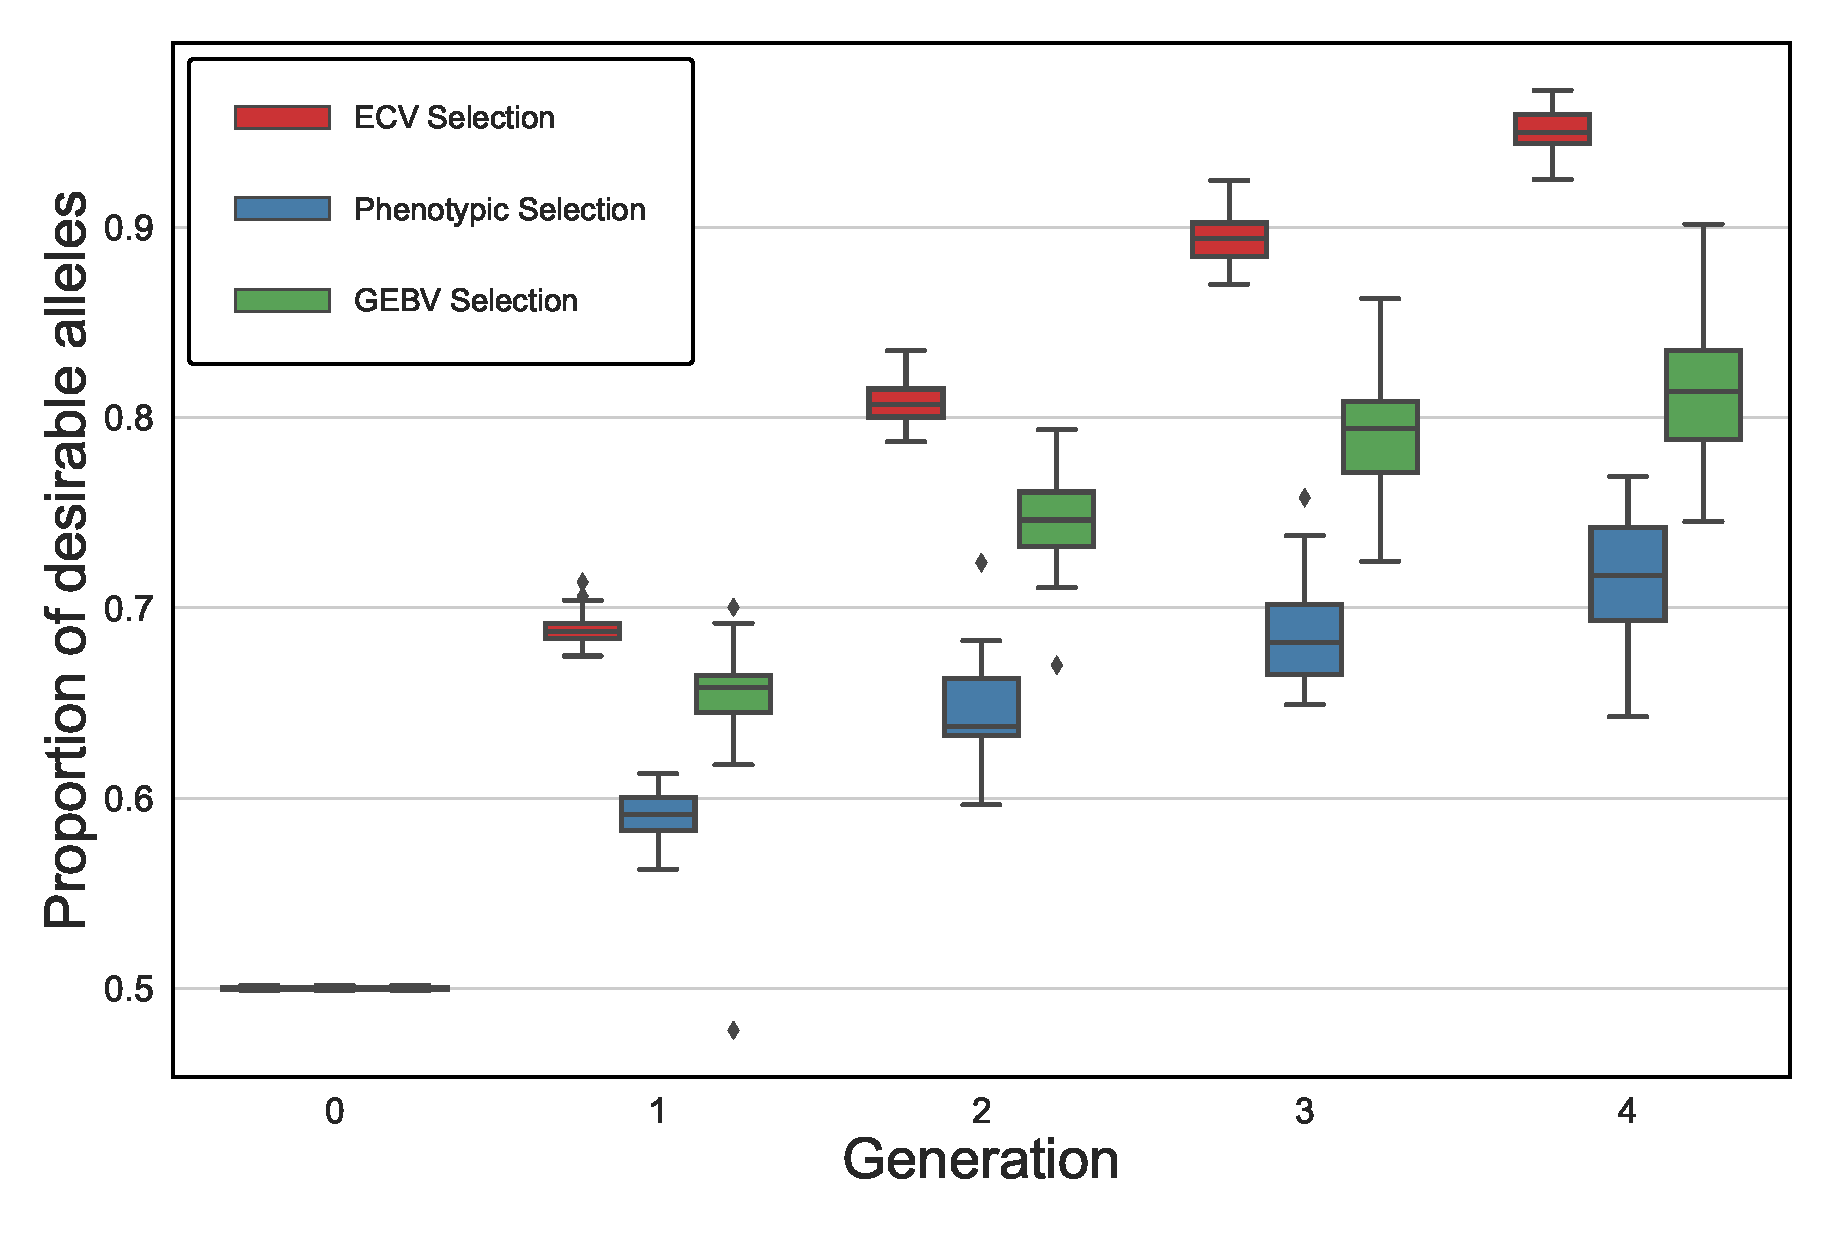
\includegraphics[scale=0.3]{Figures/SO_proportion.eps}
    \caption{Proportion of desirable alleles for Trait 1}\label{fig.1a}
    \end{subfigure}\\
     \begin{subfigure}[h!t]{\textwidth}
     \centering
    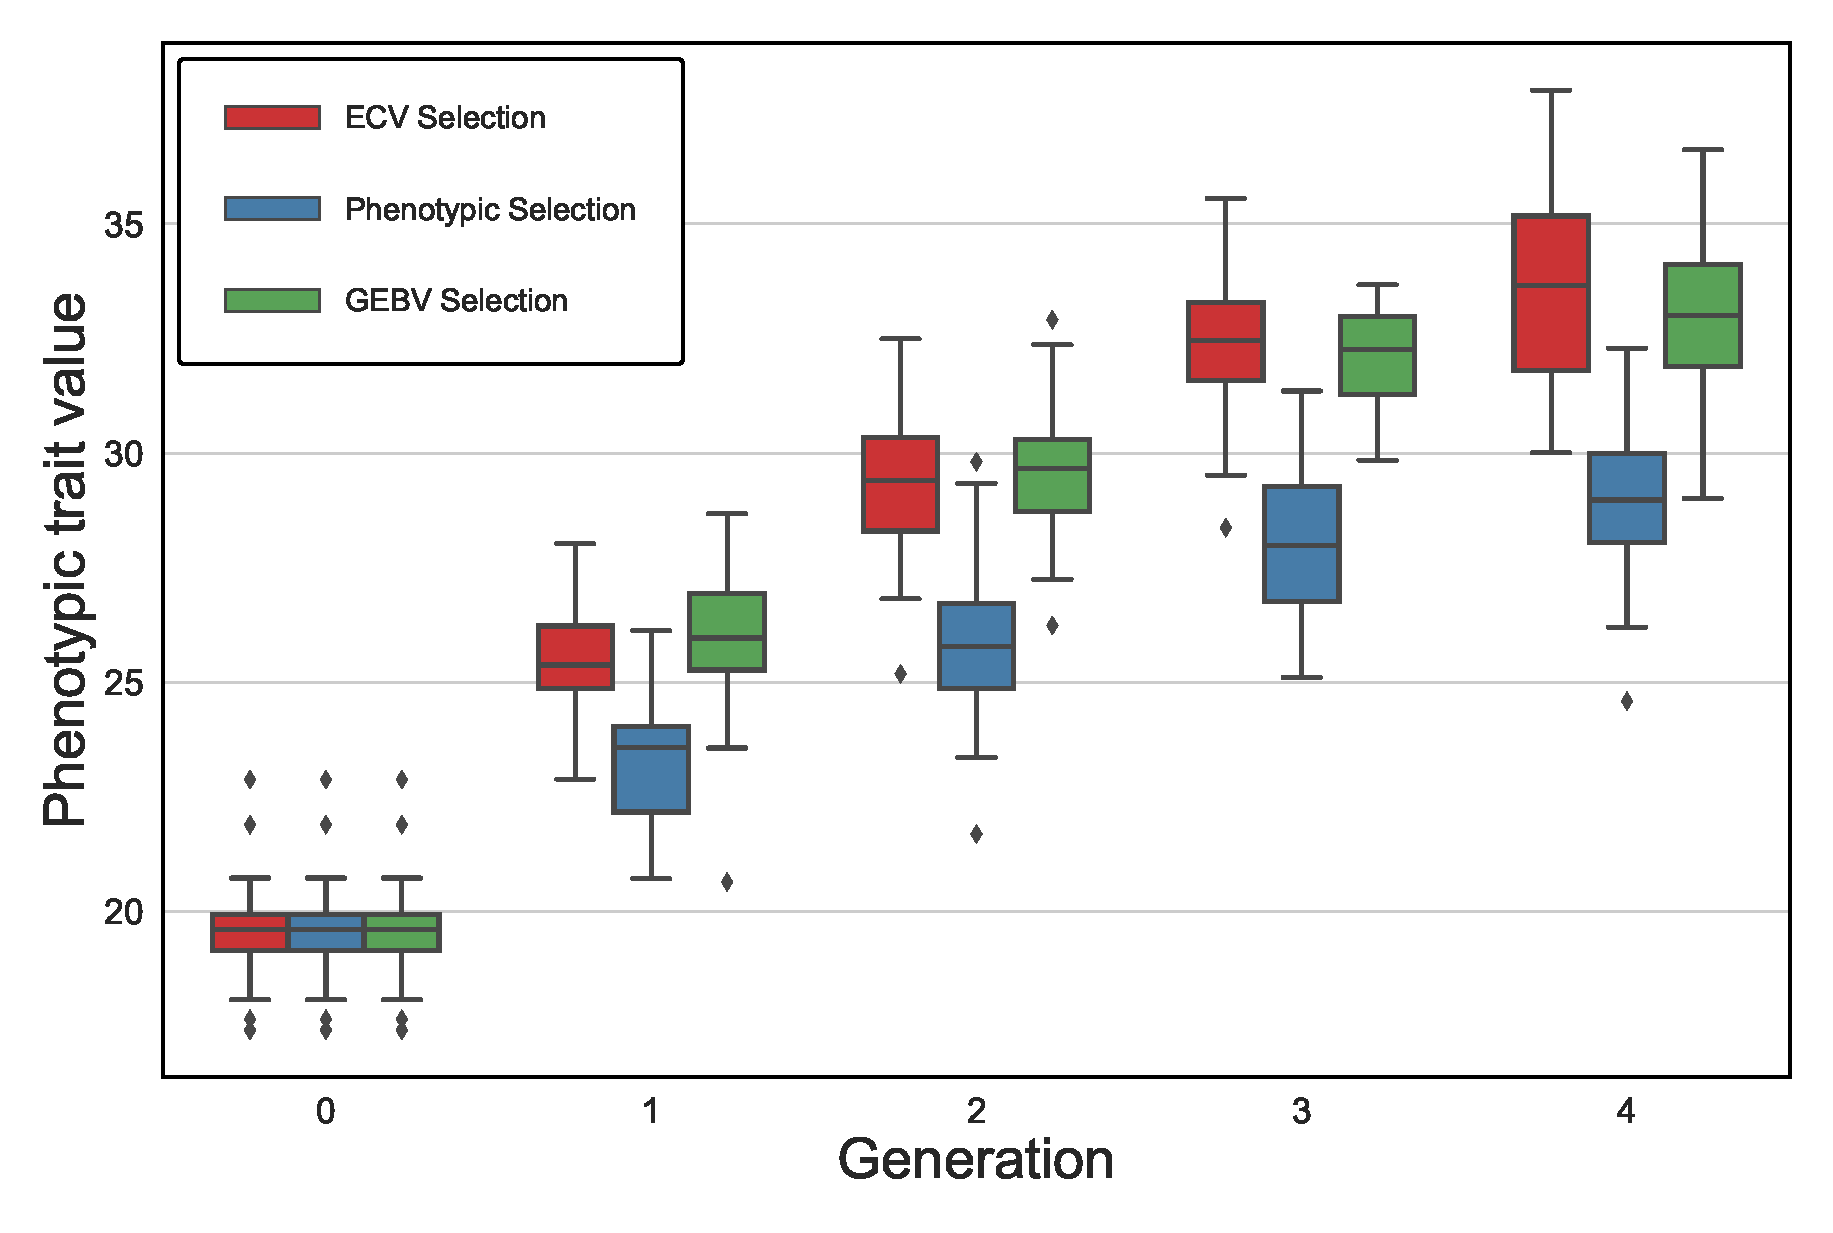
\includegraphics[scale=0.3]{Figures/SO_pheno_values.eps}
    \caption{Phenotypic trait value for Trait 1}\label{fig.1b}
    \end{subfigure}\\
    \begin{subfigure}[h!t]{\textwidth}
    \centering
    \includegraphics[scale=0.3]{Figures/SO_inbreeding.eps}
    \caption{Genomic relatedness of selected parents}\label{fig.1c}
    \end{subfigure}
    \caption{Performance of ECV, phenotypic and GEBV selection methods in 30 simulation runs for single trait improvement}
    \label{fig:SO_results}
\end{figure*}


Single-trait optimization does not guarantee improvement for phenotypes other than the target trait. Figure~\ref{fig:SO_other_traits} shows boxplots for Trait 2 and Trait 3 when we optimize Trait 1 in a single-trait optimization framework. The frequency for the desirable allele (Figure~\ref{fig.2a}) as well as the phenotypic values (Figure~\ref{fig.2b}) remained unimproved for Trait 2. The scenario could be worse if target traits are determined by QTLs with antagonistic pleiotropic effects. This can be seen in Figures~\ref{fig.2c} and~\ref{fig.2d}, which depict a significant decrease in the proportion of desirable alleles and phenotypic values of Trait 3 as a result of optimizing for Trait 1. 

%Furthermore, Trait 3 which is negatively correlated with trait 1, showed a significant decrease in terms of both proportion of desirable alleles (Figure 2(c)) and the trait values (Figure 2(d)), when . 

%Breeders routinely make decision based on more than one phenotype (ref1). Adequately selecting parents for population advancement simultaneously considering multiple traits possesses a greater challenge, because the improvement of one trait will cause concurrent changes for other traits in correlations (ref2). For example, changes in proportion of desirable allele and phenotypic values of the progeny of Trait 2 and Trait 3 were depicted in Figure~\ref{fig:SO_other_traits}. Owing to the negative correlation, a significant decrease in terms of proportion of desirable alleles and phenotypic values of Trait 3 was seen as a result of selecting for Trait 1, when selection was performed on individual phenotypes.

%\alert{the old stuff here}
%Single-trait optimization does not guarantee any improvement for any phenotype trait other than the target trait. Thus, in a multiple trait breeding program, when a trait is negatively correlated with the target trait, the single-trait optimization might not provide enticing results for that trait. Figure~\ref{fig:SO_other_traits} shows boxplots for trait 2 and trait 3 when we optimize trait 1 in a single trait optimization framework based on the ECV. We observe that the trait 2 does not show any improvement through four generations. Furthermore, trait 3 which is negatively correlated with trait 1, shows a significant decrease in terms of both proportion of desirable alleles and the trait values. 

\begin{figure*}[htb!]
    \centering
   \begin{subfigure}[h!t]{0.45\textwidth}
        \centering
    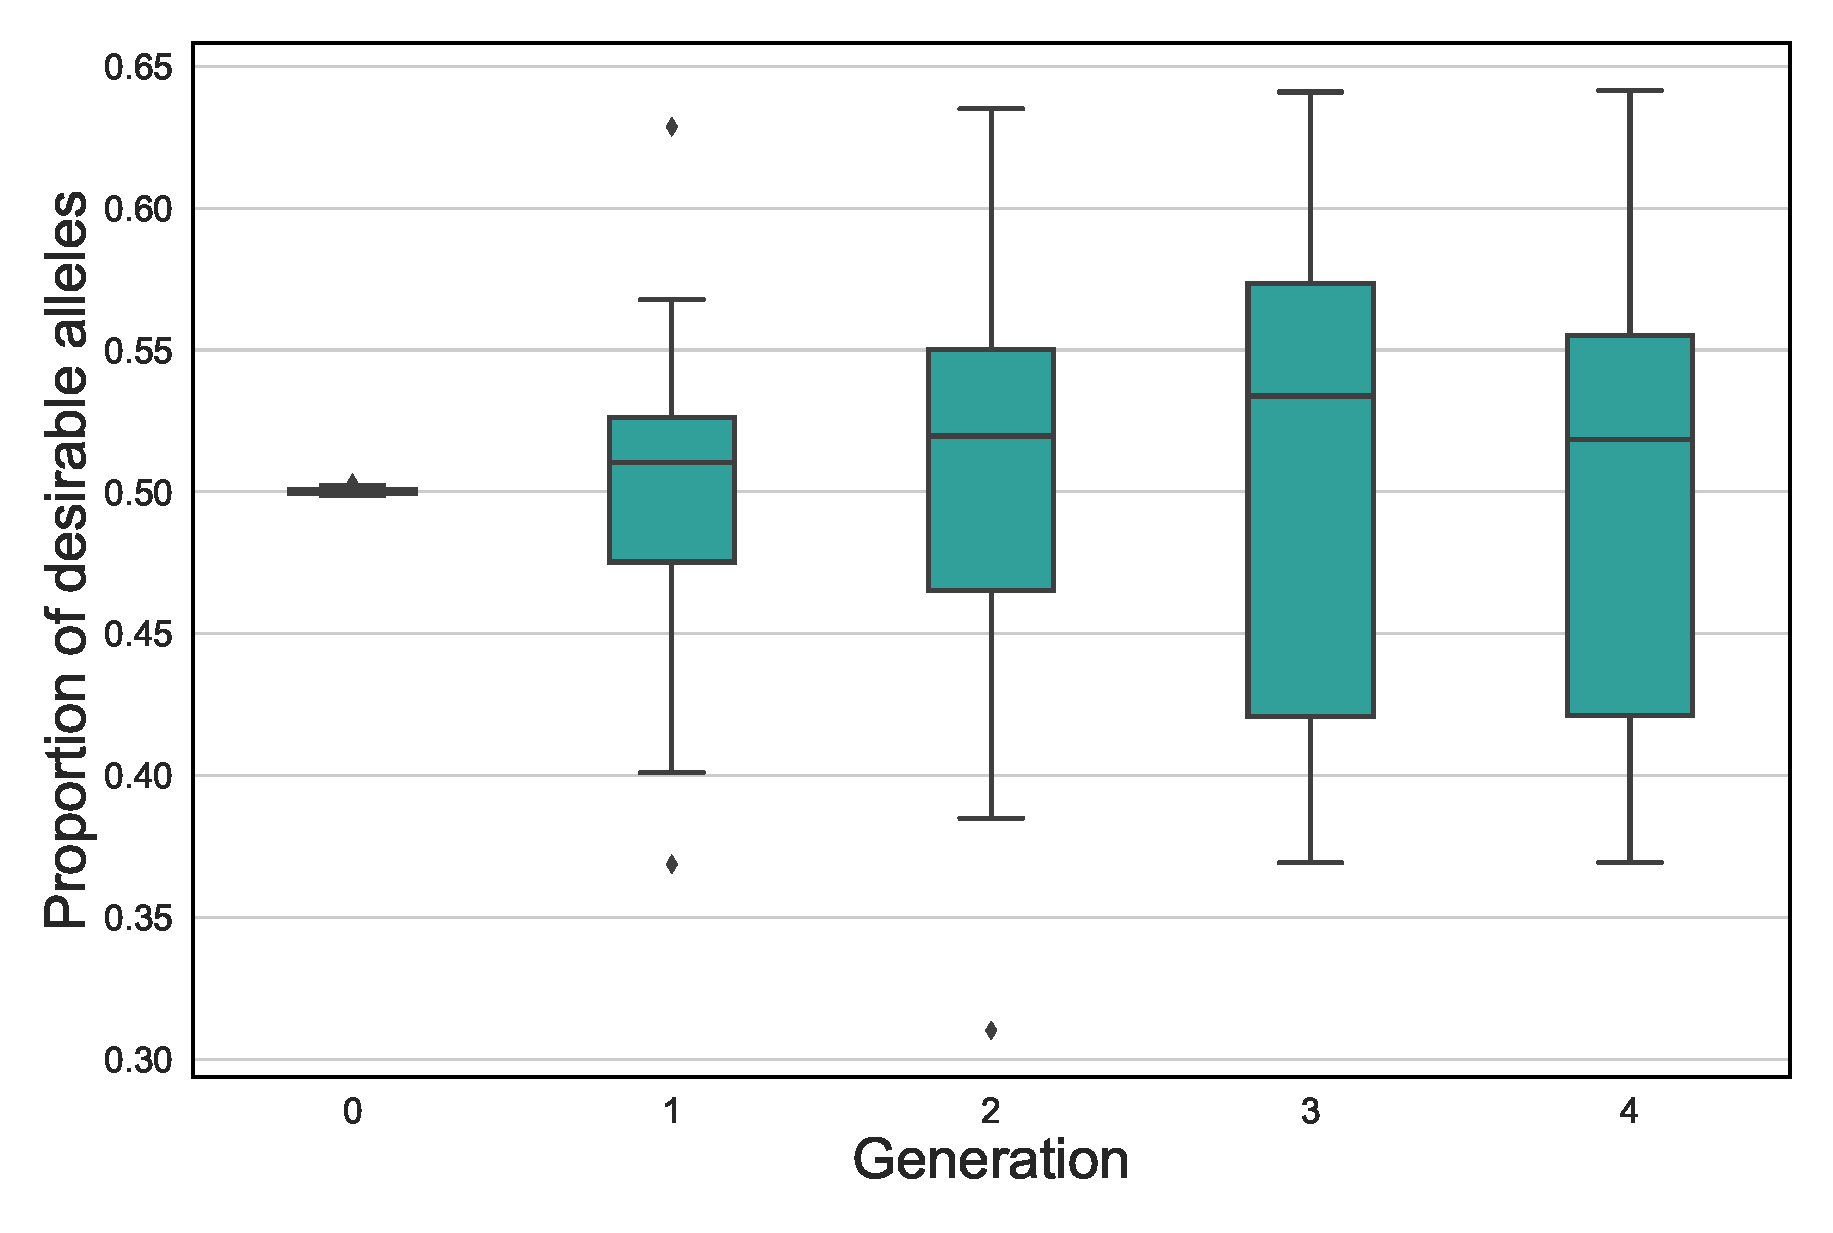
\includegraphics[scale=0.25]{Figures/SO_proportion_trait2_case.eps}
    \caption{Proportion of desirable alleles for Trait 2}\label{fig.2a}
    \end{subfigure}
    \hfill
     \begin{subfigure}[h!t]{0.45\textwidth}
        \centering
    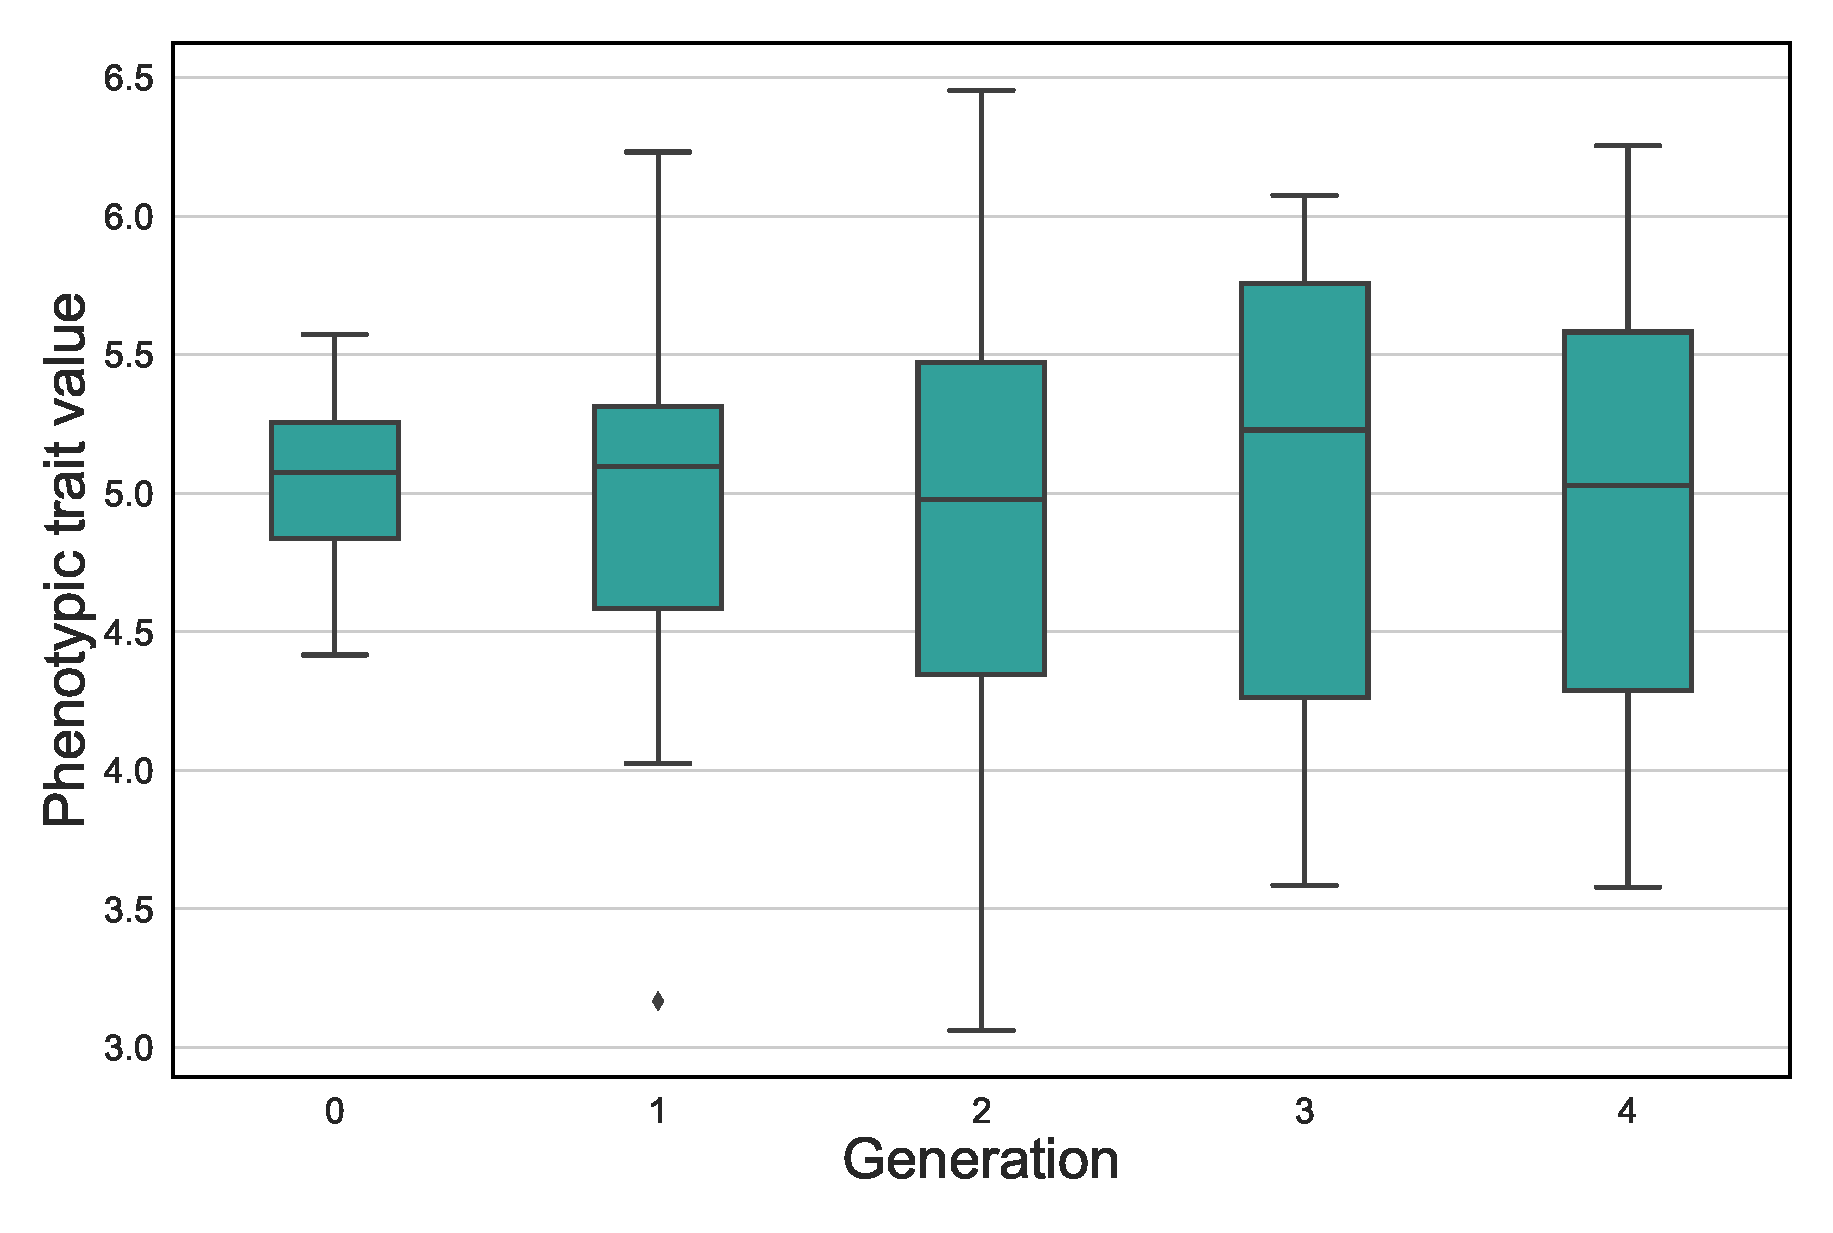
\includegraphics[scale=0.25]{Figures/SO_pheno_trait2_case.eps}
    \caption{Phenotypic trait values for Trait 2}\label{fig.2b}
    \end{subfigure}\\
    \begin{subfigure}[h!t]{0.45\textwidth}
        \centering
    \includegraphics[scale=0.25]{Figures/SO_proportion_trait3_case.eps}
    \caption{Proportion of desirable alleles for Trait 3}\label{fig.2c}
    \end{subfigure}
    \hfill
    \begin{subfigure}[h!t]{0.45\textwidth}
        \centering
    \includegraphics[scale=0.25]{Figures/SO_pheno_trait3_case.eps}
    \caption{Phenotypic trait values for Trait 3}\label{fig.2d}
    \end{subfigure}
    \caption{Effect of improving Trait 1 on the performance of Trait 2 and Trait 3 based on proportion of desirable alleles and phenotypic trait value.}
    \label{fig:SO_other_traits}
\end{figure*}

For multi-trait parental selection based on ECV, we employed the lexicographic multi-objective optimization approach described earlier. The tolerances were chosen based on  preliminary experiments as follows: let $\tau_{i,j}$ denote the degradation tolerance for optimization objective $i$ in generation $j$, then we used $\tau_{1,0}=0.17, \tau_{1,1}=0.05 , \tau_{1,2}=0.05 , \tau_{1,3}=0.05$ and $\tau_{2,0}=0.00, \tau_{2,1}=0.00 , \tau_{2,2}=0.00 , \tau_{2,3}=0.05$. In general, the tolerance parameters can be calibrated to have the desired impact on the model. The results in Figure~\ref{fig:MO_results} show the advantage of using ECV. Despite the negative genetic correlation, ECV was able to increase the desirable allele frequency to $0.70$ ($\pm0.02$), $0.65$ ($\pm0.08$), and $0.72$ ($\pm0.01$), for Trait 1, Trait 2, and Trait 3, respectively. In contrast, the impact of negative correlation between Trait 3 and Trait 1 was most obvious when the phenotypic selection was used, leading to a significant loss of desirable allele for Trait 1 (see Figure~\ref{fig.3a}). Similarly, ECV improved phenotypic values of the progeny for all traits simultaneously, whereas no improvement for Trait 1 and Trait 2 was found using phenotypic selection in our simulations when the tolerances were set slightly favoring Trait 3. It is noteworthy that a genomics-informed selection method, GEBV, returned comparable results to ECV for Trait 1. This benefit of GEBV, however, is at the expense of genetic diversity, as shown in Figure~\ref{fig:MO_inbreeding}. 

\begin{figure*}[htb!]
    \centering
   \begin{subfigure}[h!t]{0.4\textwidth}
        \centering
    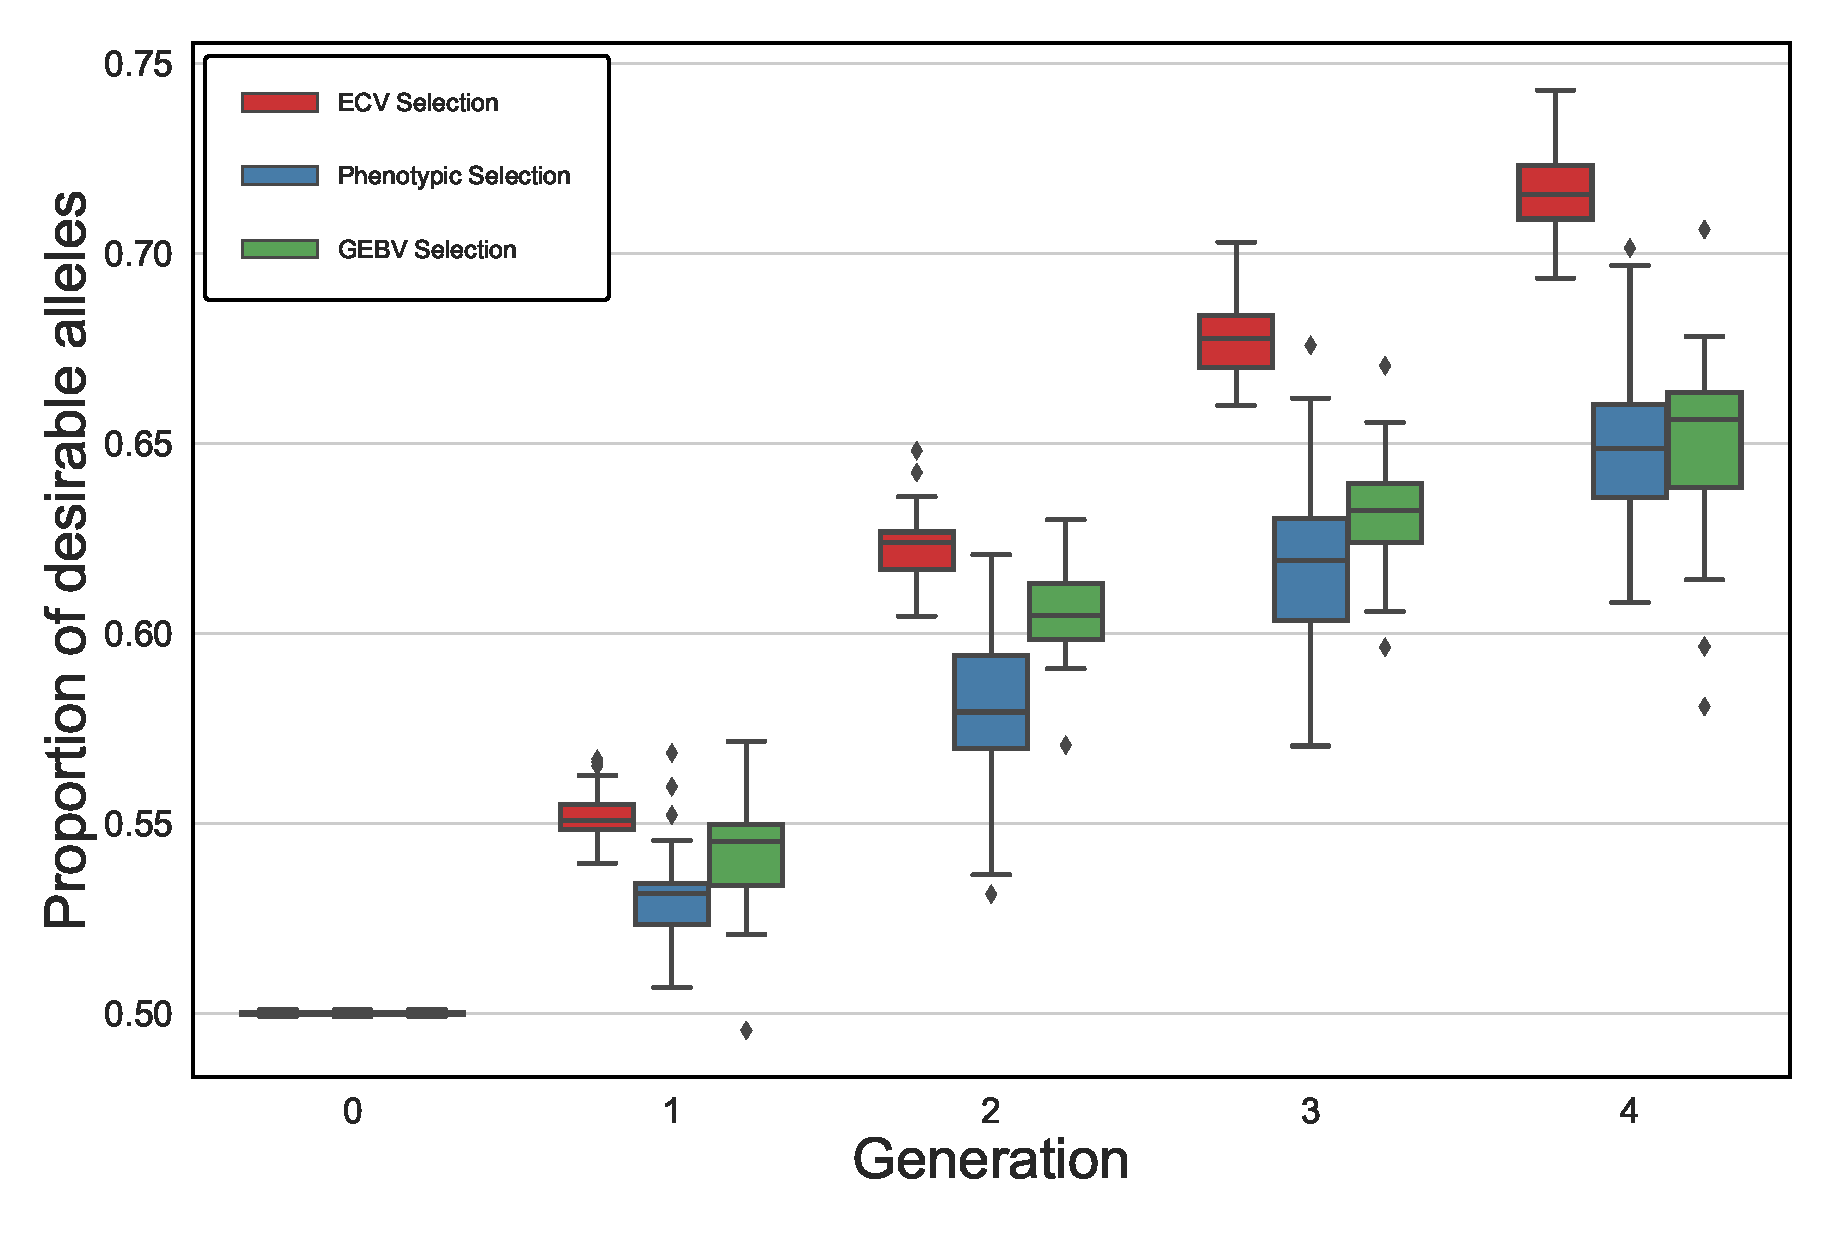
\includegraphics[scale=0.25]{Figures/MO_proportion_trait3.eps}
    \caption{Proportion of desirable alleles for Trait 3}\label{fig.3a}
    \end{subfigure}
    \hfill
    \begin{subfigure}[h!t]{0.4\textwidth}
    \centering
    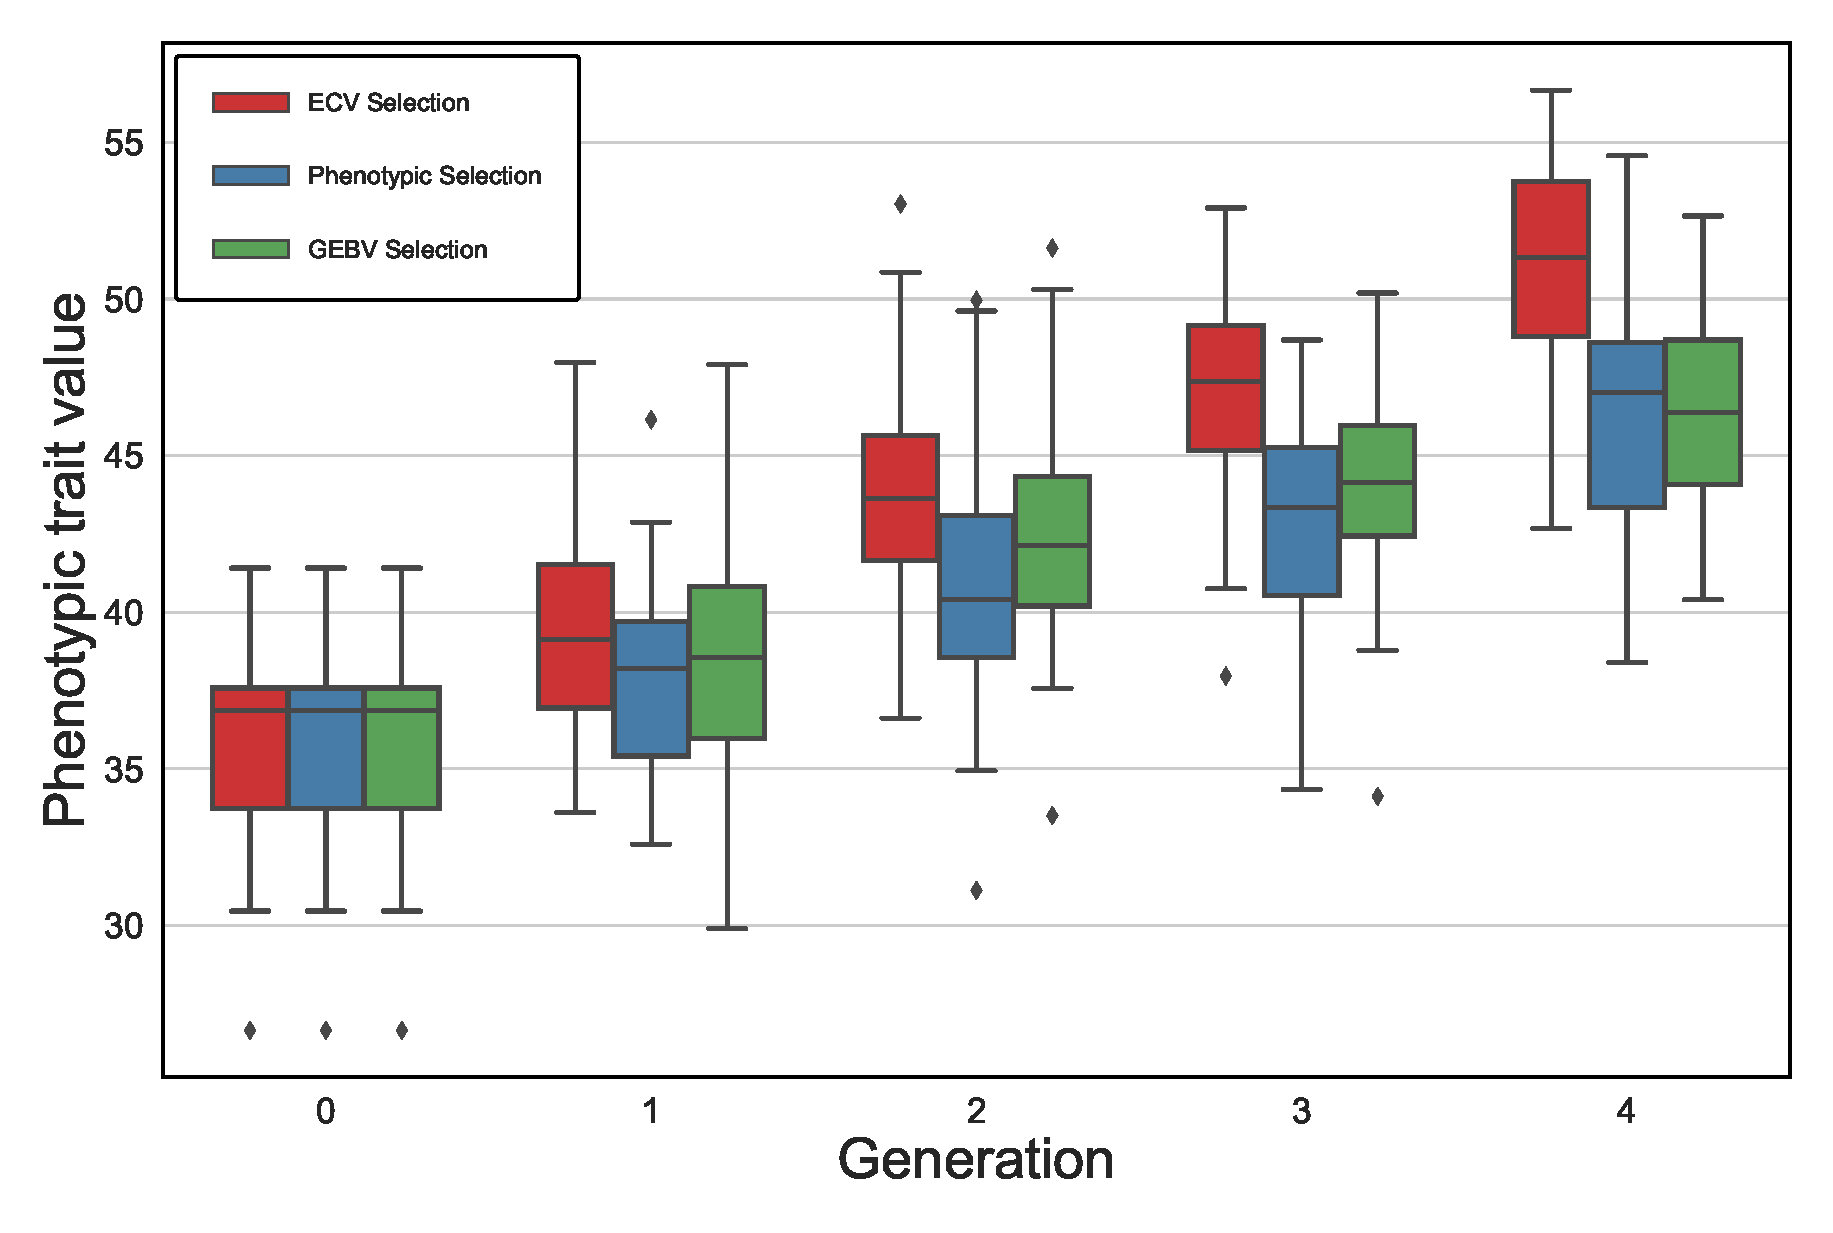
\includegraphics[scale=0.25]{Figures/MO_pheno_values_trait3.eps}
    \caption{Phenotypic trait values for Trait 3}\label{fig.3b}
    \end{subfigure}
    \\
      \begin{subfigure}[h!t]{0.4\textwidth}
    \centering
    \includegraphics[scale=0.25]{Figures/MO_proportion_trait1.eps}
    \caption{Proportion of desirable alleles for Trait 1}\label{fig.3c}
    \end{subfigure}
    \hfill
    \begin{subfigure}[h!t]{0.4\textwidth}
    \centering
    \includegraphics[scale=0.25]{Figures/MO_pheno_values_trait1.eps}
    \caption{Phenotypic trait values for Trait 1}\label{fig.3d}
    \end{subfigure}
    \\
    \begin{subfigure}[h!t]{0.4\textwidth}
    \centering
    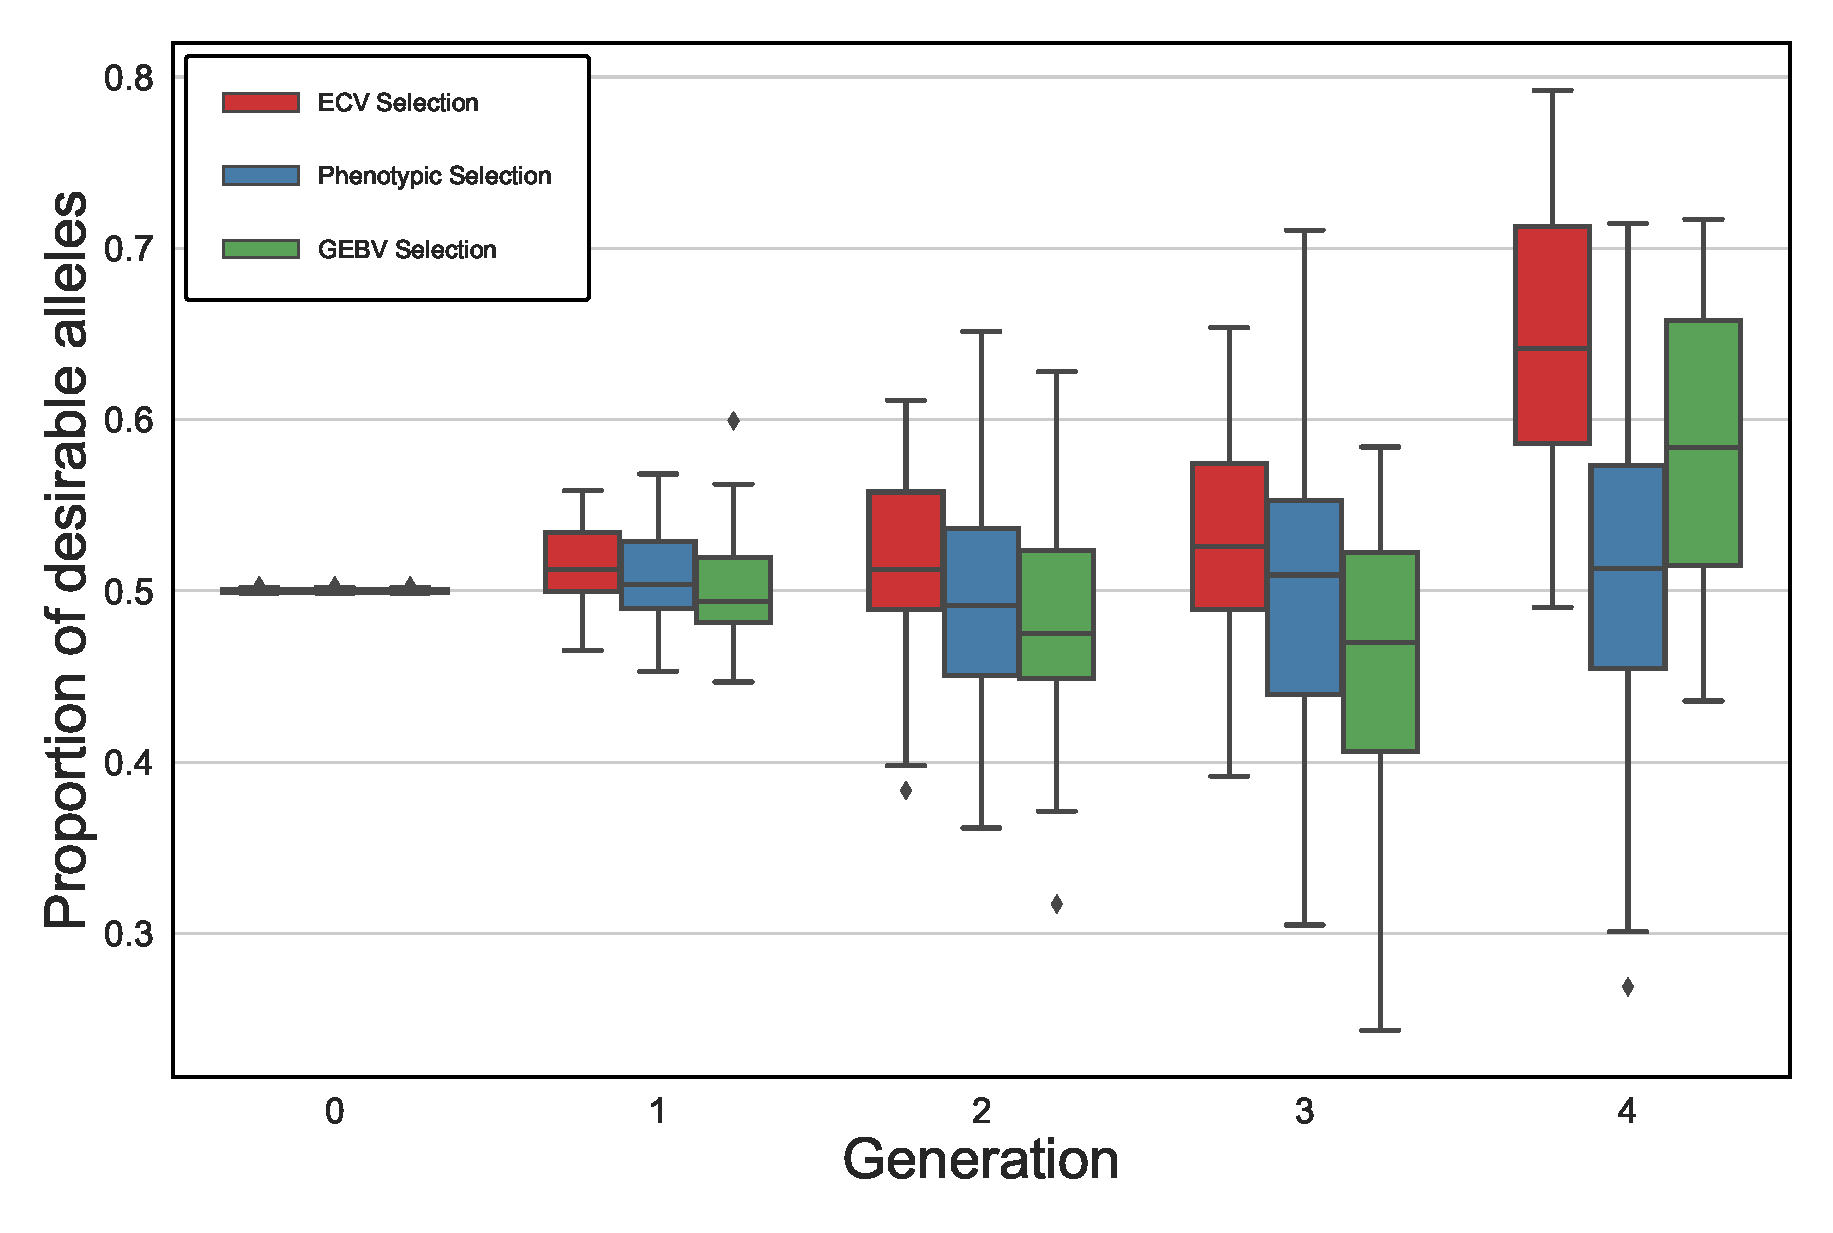
\includegraphics[scale=0.25]{Figures/MO_proportion_trait2.eps}
    \caption{Proportion of desirable alleles for Trait 2}\label{fig.3e}
    \end{subfigure}
    \hfill
    \begin{subfigure}[h!t]{0.4\textwidth}
    \centering
    \includegraphics[scale=0.25]{Figures/MO_pheno_values_trait2.eps}
    \caption{Phenotypic trait values for Trait 2}\label{fig.3f}
    \end{subfigure}
    \caption{Performance of ECV, phenotypic and GEBV selection methods in $30$ simulation runs for multiple trait improvement}
    \label{fig:MO_results}
\end{figure*}

\begin{figure}[ht!]
    \centering
    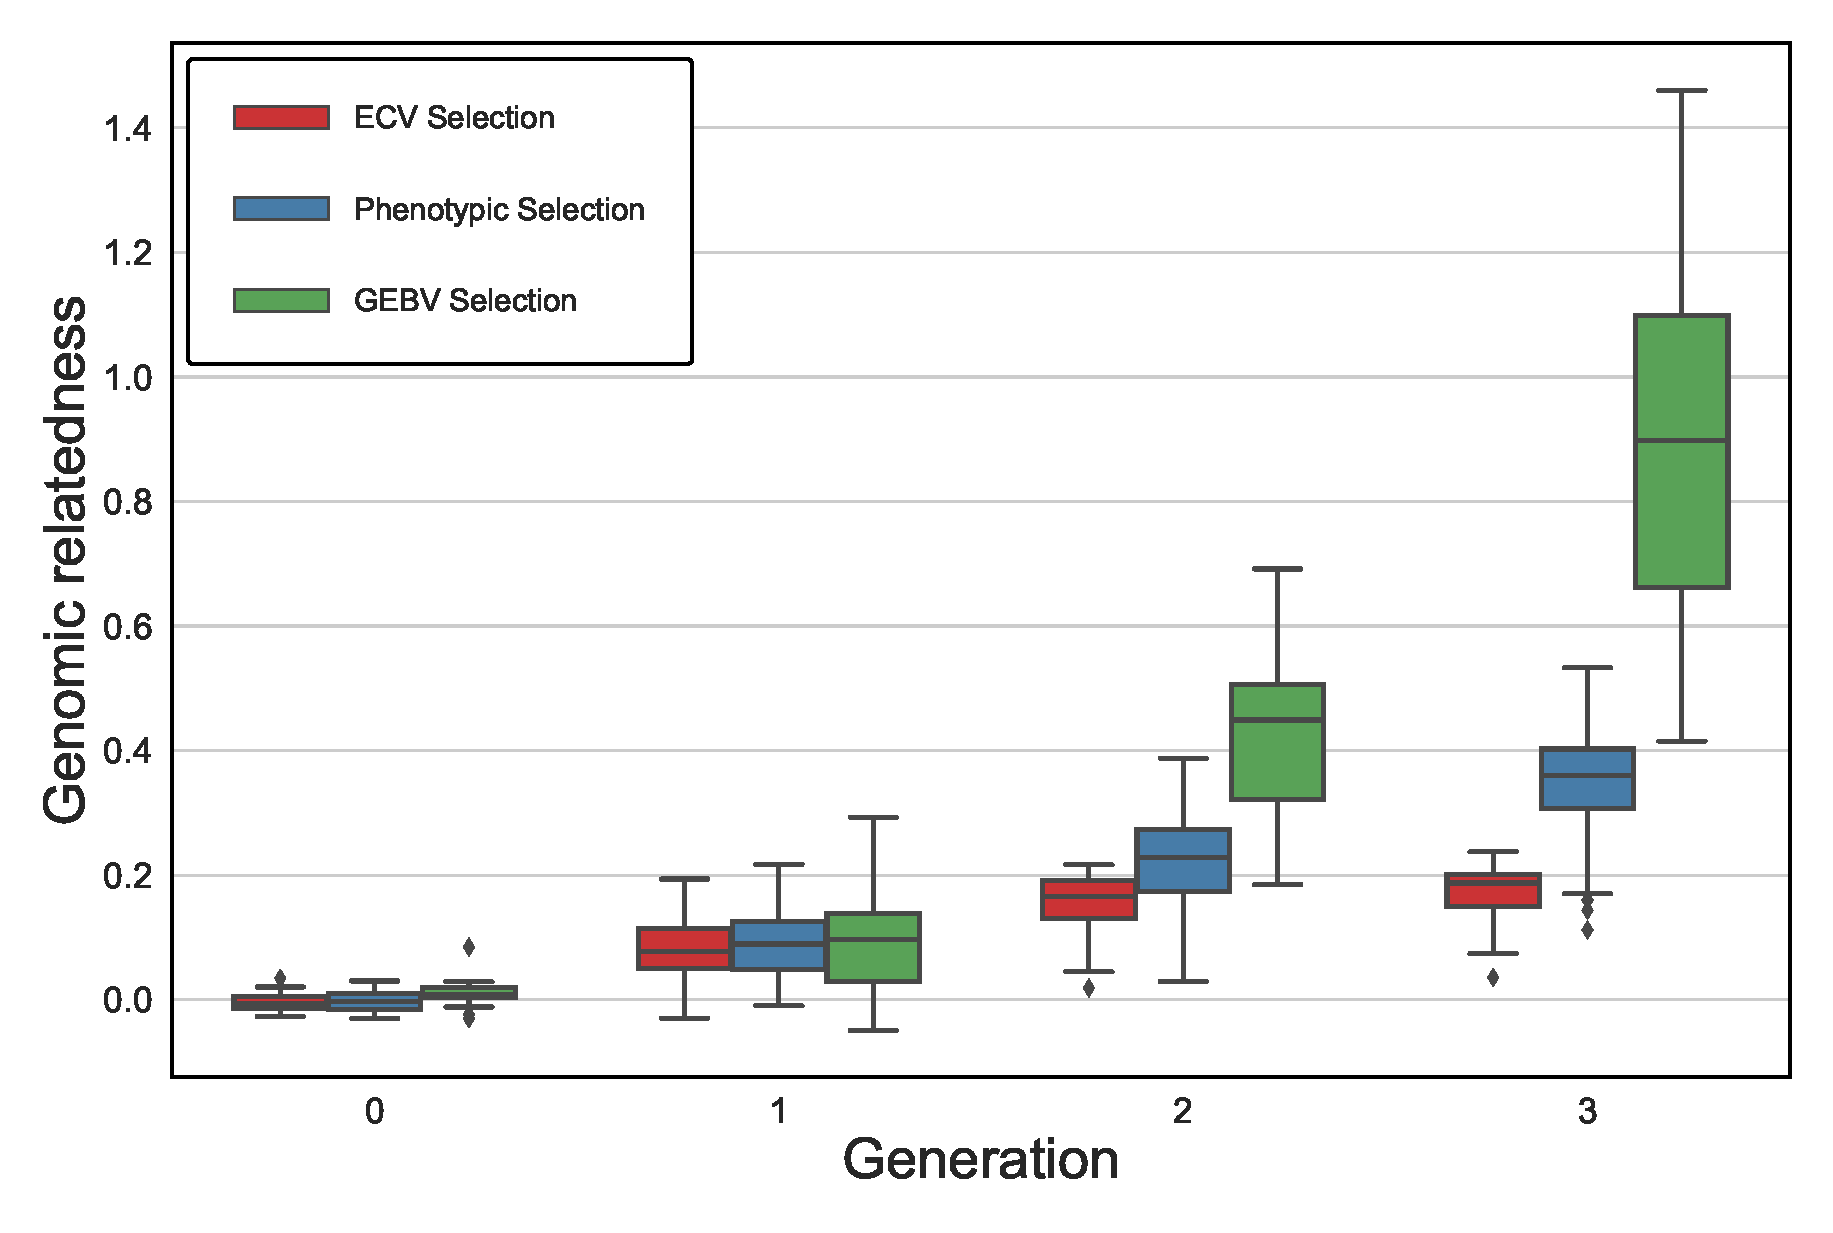
\includegraphics[scale=0.4]{Figures/MO_inbreeding.eps}
    \caption{Genomic relatedness for multiple trait improvement based on ECV, phenotypic and GEBV selection methods}
    \label{fig:MO_inbreeding}
\end{figure}

%--------------------------------------%
\section*{Discussion}\label{sec:discussion} %%% 1519 words

The principal objective of breeding is to combine as many desirable traits as possible into a single individual. For example, in plant breeding the breeders are tasked with developing elite genotypes that display desirable end-use characteristics, disease resistance, and also are well-adapted to a range of environmental conditions~\citep{Breseghello2013}. These desirable characteristics are typically possessed by multiple founders. By mixing and recombining founder genomes, the distribution of these desirable phenotypes observed in the offspring, owing to the segregation of genes and QTLs, allow breeders to identify superior individuals for advancement. 

However, when these desired characteristics differ in variability, heritability, economic importance, and are correlated among other phenotypes and genotypes, effective mating designs capable of improving multiple traits simultaneously can be challenging to identify~\citep{johnson1988model}. This breeding process is also ineffective as breeders tend to make hundreds or thousands of crosses, of which only a few are advanced in the subsequent years~\citep{witcombe2013plant}. Traditionally, these objectives are achieved by breeding from the ``best''---the best being determined by their own phenotypic values (Allard 1999; Akdemir et al. 2018). More advanced techniques, such as pedigree-based~\citep{henderson1984applications, gianola1986bayesian}, marker-based genetic value predictions~\citep{lande1990efficiency, hospital1997marker, bernardo2006usefulness}, and mating designs by genomic information~\citep{akdemir2016efficient} are also  available. The capacity to derive an optimal subset to refine mate selection has been discussed~\citep{akdemir2016efficient, han2017predicted}. \cite{jansen1985selecting} addressed the issue of factorial growth in the number of combinations of males and females to cross by formulating and solving an integer programming model to improve the overall progeny merit. When the breeding objective involves more than one trait, a selection index of progeny merit was considered as a linear function of estimated breeding values for each trait by~\cite{allaire1980mate}. In animal breeding, for instance, the genetic merit of calves is estimated as half of the sire's and half of the dam's breeding value. An optimization based procedure for mate selection in animal breeding is introduced in~\citep{kinghorn1998mate, kinghorn2011algorithm} based on a mate selection criterion  proposed by~\cite{kinghorn199919}.  

In the genomics era, the parental selection problem has been increasingly addressed with the use of genomic relationships~\citep{sun2013mating}, heuristic searches for gene pyramiding~\citep{de2015heuristic}, and by modeling the recombination of desirable alleles as a result of crossing two breeding parents~\citep{han2017predicted}. \cite{han2017predicted} proposed an efficient  algorithm for calculating the PCV defined as the probability that a gamete of a random progeny from crossing two genetic individuals would consist only of desirable alleles. In a specific case where the desirable allele for the $i$-th QTL is not present in both parents (denoted by $k$ and $k'$), such that $L^k_{i,1}=L^k_{i,2}=L^{k'}_{i,1}=L^{k'}_{i,2}=0$, PCV will conclude that the $i$-th component of gamete $g^3$ is zero with probability one and hence $PCV(L^k,L^{k'},r,\alpha_0)=0$. In this case, the individuals $k$ and $k'$  will not be selected, regardless whether or not there maybe be desirable alleles present in the rest of the chromosome. In an extreme case of $i=1$, and individuals $k$ and $k'$ carrying the desirable alleles in all remaining QTLs ($i\not=1$), the cross between $k$ and $k'$ is, in fact, the best candidate for genetic improvement that PCV will be unable to recognize. Further, considering the polygenic inheritance of agronomical performance traits~\citep{lynch1998genetics, scott2021limited}, the PCV approaches zero for all breeding parents as the number of QTL increases. Consider the following probabilistic inequality (Fr\'echet inequality):
\begin{equation}\label{eq:upperbound}
   \PCV(L^k,L^{k'},r,\alpha_0=0.5) = \Pr\big(g^3_i=1\ \forall i\in[N]\big)\le \min_{i\in[N]}\Pr(g^3_i=1).
\end{equation}
Hence, the larger the value of $N$, the greater the chance  $L^k_{i,1}=L^k_{i,2}=L^{k'}_{i,1}=L^{k'}_{i,2}=0$ for some QTL $i$. The PCV method could therefore lead to indiscriminate mate selection for traits that have hundreds or thousands of underlying QTLs because the PCV value is (nearly) zero for essentially any choice of mates. This observation  motivated us to introduce our  ECV criterion as a ``risk neutral'' alternative to PCV. As Figure~\ref{fig.1a} shows, our results demonstrated a significantly greater capacity to increase desirable allele frequency compared to the conventional phenotypic selection and the selection done by the genomics-derived GEBV; and, the benefit of using ECV can be realized in as short as two generations. Moreover, the greater range of trait value distribution presents additional opportunities for breeders to identify the superiors for population advancement (see Figure~\ref{fig.1b}).

%to address these drawbacks of mate selection for polygenic traits. 

%\bb{Our primary technical contributions are in Theorems~\ref{thm.ecv} and~\ref{thm.ecv_multi-trait} that provide closed-form analytical expressions for the expected value, which subsequently allows us to employ them in an optimization framework.} Furthermore, as Figure~\ref{fig.1a} shows, our results demonstrated a significantly greater capacity to increase desirable allele frequency compared to the conventional phenotypic selection and the selection done by the genomics-derived GEBV. The \replaced{benefits of using ECV-optimal parental selection (ECV-OPS)}{benefit of ECV} can be \replaced{realized}{identified} in as short as two generations. Moreover, the \deleted{resultant} greater range of trait value distribution \replaced{resulting from ECV-OPS}{of ECV's} \bb{[apostrophe doesn't seem right here: do we wanna call the results of our approach ECV-OPS; use ECV for just the metric/objective, not the method/approach]} presents additional opportunities for breeders to identify the superiors for population advancement (see Figure~\ref{fig.1b}). 

Based on our simulations, we observe that the breeding population has gone from unrelated to essentially full-sibs in three generations of selecting breeding parents based on GEBVs (see Figure~\ref{fig.1c}). Compared to the phenotypic selection, GEBV selection might have manifested a rapid increase of relatedness by crossing individuals closely related to the training population~\citep{bassi2016breeding, forutan2018inbreeding}. Though GEBV selection might show a capacity to provide short-term genetic gain, selecting breeding parents solely by GEBVs would lead to undesirable consequences such as loss of genetic diversity, further diminishing long-term genetic gain~\citep{jannink2010dynamics, doekes2018trends}. 

To ensure the capacity to preserve multiple genetic lineages, ECV allows for the selection of more than one pair of individuals, and while self-crossing was not allowed in this study, our method permitted the same individual to be crossed with multiple breeding parents as long as the genomic relationship of the parents was not greater than $\epsilon$, a parameter that breeders can use to control how much inbreeding is acceptable. 

Fundamental to all variety improvement programs is the identification of the most efficient path to reach breeding objectives~\citep{bernardo2002breeding, akdemir2019multi}. However, breeders are usually tasked with combining a suite of traits in addition to yield and growth components. The negative genetic correlations caused by the non-random association of alleles underlying these breeding objectives impose additional challenges, as selecting based on one trait may adversely impact another~\citep{lynch1998genetics}. To simultaneously improve multiple traits, phenotype-based selection indices have been widely considered~\citep{hazel1942efficiency, hazel1994selection, villanueva1997optimization, jannink2000index, moeinizade2020multi}. Selecting breeding parents based on a selection index does not necessarily choose the best genetics to recombine; further, since the selection index applied is a weight assignment of target phenotypes, such decisions could result in the loss of beneficial alleles. 

In this study, the proposed ECV framework is based on an allele introgression process. Rather than relying on the phenotypes of breeding parents, ECV identifies the crosses with the highest likelihood of transmitting desirable alleles to the progeny. In the case where multiple traits need to be considered simultaneously, ECV seeks the optimal combination of alleles for all target phenotypes ordered by their importance, while maintaining a customizable tolerance  such that QTLs with antagonistic pleiotropic gene action could remain in consideration before the final breeding recommendation is made. Figure~\ref{fig:MO_results} shows that despite the negative correlation between Traits 1 and 3, ECV was able to increase desirable allele frequency for all traits in our simulation studies. In addition, as seen from Figure~\ref{fig:MO_inbreeding}, the inbreeding coefficient in the progeny was regulated as ECV was optimized with the tolerance constraint on the genomic relatedness between breeding parents. As genotyping has become routine in breeding programs~\citep{hayes2010genome, bentley2022frontiers}, the application of this constraint ought to be considered to mitigate the multiple trait scenario in Figure~\ref{fig:MO_results}, where the gain might be built at the expense of genetic diversity (Figure~\ref{fig:MO_inbreeding}), a phenomenon also found in index selection methods~\citep{akdemir2019multi}. If practical considerations favor breeding parents to be selected from a narrow genetic pool, the constraint could be moved to the objective as a penalty term. 

Breeding programs develop elite genotypes that often demonstrate similar essential genomic profiles of desirable end-use characteristics, agronomical attributes, disease resistance packages, as well as adaptation to the target environment. Breeding among the elites can produce new variability as the source of new cultivars with minimal risk of introducing undesirable features. This variation may eventually be exhausted, and new genes and alleles must be introduced. Identifying beneficial alleles from un-adapted material itself has been described as searching for a needle in a haystack~\citep{pixley2014seeds}. Introgressing these novel alleles can also be risky because the unwanted alleles in exotic germplasm may distrupt essential  allele combinations~\citep{willcox2022mining}; and, it requires a higher institutional cost due to a greater number of crosses and longer breeding cycle needed to achieve the breeding objectives~\citep{snelling2019genetic, neyhart2019multi}. Based on our simulations, we reckon that ECV can be an option. 

Beyond animal and cereal crop breeding, we suspect that implementing optimization-based methods like ECV could be advantageous to breeding of genetically diverse, long-generation, and slow reaction, cross-pollinated species, such as conifers. Tree breeders generally establish open-pollinated seed orchards for selection~\citep{white2007forest}, and several mating designs have been proposed~\citep{nakoonctextordmasculine1976multiple, zobel1984applied}, among which the polycross is considered as one of the most cost-effective~\citep{kumar2007testing, lenz2020genomic}. The ability to design the pollen pool while managing inbreeding with ECV will provide the capacity to rapidly increase desirable allele frequencies and, at the same time, avoid severe inbreeding depression for conifer species~\citep{berry2014genetics, mwansa2002multiple, snelling2019genetic}. 

The conceptual framework we have introduced and our results show that adopting multi-objective optimization tools from operations research to solve breeding problems is highly advantageous~\citep{cameron2017systematic, beans2020inner, kusmec2021interdisciplinary}. Several improvements or extensions suggested next should also be considered. When the pool of genetic diversity increases, solving integer programming problems for ECV will require further development to account for different distributions of crossover events in different crosses~\citep{stapley2017variation,nachman2002variation,jabbari2019common,dreissig2019variation}. Furthermore, as multi-parent populations like MAGIC (multi-parent advanced generation inter-cross) have become a means to provide germplasm for breeding programs~\citep{scott2020multi}, there is a need to expand optimization frameworks such as ECV to consider multiple parental lineages, which might also help guide the polycross mating design in forestry~\citep{frandsen1940some, lambeth2001polymix}. 

%\hl{On the other hand, adding variance of cross value to the objective function, which includes the expectation of cross value, will result in a risk-averse problem that might be worth studying but will also increase the complexity of the objective function and the overall computational complexity.} \bb{[I get the idea here, but I am not sure one sentence is enough to make the point. What constitutes risk in this setting? Does the loss function we use continue to make sense if we are talking about risk of downside loss and variance minimization? In other words, are we saying that there is a chance of high variance resulting from  our recommendations for crossing? Do we observe that in our results? Going from PCV to ECV to a mean-variance model is natural to us OR folks, but we need to ease a general audience into that concept. Is this necessary at this point in the paper? Feel like we are throwing open a big topic without sufficient guardrails and too abruptly.]}

%--------------------------------------%
\section*{Acknowledgements}\label{sec:thanks}
%%% 97 Around words

Funding for this work was supported by grants from the Oklahoma Wheat Research Foundation (for CC), Oklahoma Center for the Advancement of Science and Technology (OCAST) award number PS15-011-2 and PS19-004 for CC. This work was completed utilizing the High-Performance Computing Center facilities of Oklahoma State University at Stillwater, and also in part by the Extreme Science and Engineering Discovery Environment (XSEDE), which is supported by National Science Foundation grant number ACI-1548562. Specifically, it used the Bridges system, which is supported by NSF award number ACI-1445606, at the Pittsburgh Supercomputing Center (PSC) under the resource allocation MCB-180177. 

\paragraph{Author contributions.} 
%%% Around 37 words
BB, JB, and CC were responsible for the conceptualization of the study. PA developed the theoretical results and computer implementations as part of his thesis. PA and CC performed the analysis and wrote the original draft. All authors contributed to interpreting results, providing feedback, and editing and approving the manuscript. 
%--------------------------------------%
\paragraph{Conflict of interest.}

The authors declare that they have no conflict of interest.
%--------------------------------------%
\section*{Data Archiving}\label{sec:data}

The data is available at the following repository: \texttt{github.com/transgenomicsosu/ECV\textunderscore Optimization}

%--------------------------------------%
\section*{Figure Legends}\label{sec:legends}

Figure 1: Performance of ECV, phenotypic and GEBV selection methods in 30 simulation runs for single trait improvement.

\noindent Figure 2: Effect of improving Trait 1 on the performance of Trait 2 and Trait 3 based on proportion of desirable alleles and phenotypic trait values.

\noindent Figure 3: Performance of ECV, phenotypic and GEBV selection methods in 30 simulation runs for multiple trait improvement.

\noindent Figure 4: Genomic relatedness for multiple trait improvement based on ECV, phenotypic and GEBV selection methods.

%--------------------------------------%
\begingroup
\raggedright
\bibliography{references}
\endgroup

\end{document}



